% Options for packages loaded elsewhere
\PassOptionsToPackage{unicode}{hyperref}
\PassOptionsToPackage{hyphens}{url}
%
\documentclass[
  man,floatsintext]{apa6}
\usepackage{amsmath,amssymb}
\usepackage{iftex}
\ifPDFTeX
  \usepackage[T1]{fontenc}
  \usepackage[utf8]{inputenc}
  \usepackage{textcomp} % provide euro and other symbols
\else % if luatex or xetex
  \usepackage{unicode-math} % this also loads fontspec
  \defaultfontfeatures{Scale=MatchLowercase}
  \defaultfontfeatures[\rmfamily]{Ligatures=TeX,Scale=1}
\fi
\usepackage{lmodern}
\ifPDFTeX\else
  % xetex/luatex font selection
\fi
% Use upquote if available, for straight quotes in verbatim environments
\IfFileExists{upquote.sty}{\usepackage{upquote}}{}
\IfFileExists{microtype.sty}{% use microtype if available
  \usepackage[]{microtype}
  \UseMicrotypeSet[protrusion]{basicmath} % disable protrusion for tt fonts
}{}
\makeatletter
\@ifundefined{KOMAClassName}{% if non-KOMA class
  \IfFileExists{parskip.sty}{%
    \usepackage{parskip}
  }{% else
    \setlength{\parindent}{0pt}
    \setlength{\parskip}{6pt plus 2pt minus 1pt}}
}{% if KOMA class
  \KOMAoptions{parskip=half}}
\makeatother
\usepackage{xcolor}
\usepackage{color}
\usepackage{fancyvrb}
\newcommand{\VerbBar}{|}
\newcommand{\VERB}{\Verb[commandchars=\\\{\}]}
\DefineVerbatimEnvironment{Highlighting}{Verbatim}{commandchars=\\\{\}}
% Add ',fontsize=\small' for more characters per line
\usepackage{framed}
\definecolor{shadecolor}{RGB}{248,248,248}
\newenvironment{Shaded}{\begin{snugshade}}{\end{snugshade}}
\newcommand{\AlertTok}[1]{\textcolor[rgb]{0.94,0.16,0.16}{#1}}
\newcommand{\AnnotationTok}[1]{\textcolor[rgb]{0.56,0.35,0.01}{\textbf{\textit{#1}}}}
\newcommand{\AttributeTok}[1]{\textcolor[rgb]{0.13,0.29,0.53}{#1}}
\newcommand{\BaseNTok}[1]{\textcolor[rgb]{0.00,0.00,0.81}{#1}}
\newcommand{\BuiltInTok}[1]{#1}
\newcommand{\CharTok}[1]{\textcolor[rgb]{0.31,0.60,0.02}{#1}}
\newcommand{\CommentTok}[1]{\textcolor[rgb]{0.56,0.35,0.01}{\textit{#1}}}
\newcommand{\CommentVarTok}[1]{\textcolor[rgb]{0.56,0.35,0.01}{\textbf{\textit{#1}}}}
\newcommand{\ConstantTok}[1]{\textcolor[rgb]{0.56,0.35,0.01}{#1}}
\newcommand{\ControlFlowTok}[1]{\textcolor[rgb]{0.13,0.29,0.53}{\textbf{#1}}}
\newcommand{\DataTypeTok}[1]{\textcolor[rgb]{0.13,0.29,0.53}{#1}}
\newcommand{\DecValTok}[1]{\textcolor[rgb]{0.00,0.00,0.81}{#1}}
\newcommand{\DocumentationTok}[1]{\textcolor[rgb]{0.56,0.35,0.01}{\textbf{\textit{#1}}}}
\newcommand{\ErrorTok}[1]{\textcolor[rgb]{0.64,0.00,0.00}{\textbf{#1}}}
\newcommand{\ExtensionTok}[1]{#1}
\newcommand{\FloatTok}[1]{\textcolor[rgb]{0.00,0.00,0.81}{#1}}
\newcommand{\FunctionTok}[1]{\textcolor[rgb]{0.13,0.29,0.53}{\textbf{#1}}}
\newcommand{\ImportTok}[1]{#1}
\newcommand{\InformationTok}[1]{\textcolor[rgb]{0.56,0.35,0.01}{\textbf{\textit{#1}}}}
\newcommand{\KeywordTok}[1]{\textcolor[rgb]{0.13,0.29,0.53}{\textbf{#1}}}
\newcommand{\NormalTok}[1]{#1}
\newcommand{\OperatorTok}[1]{\textcolor[rgb]{0.81,0.36,0.00}{\textbf{#1}}}
\newcommand{\OtherTok}[1]{\textcolor[rgb]{0.56,0.35,0.01}{#1}}
\newcommand{\PreprocessorTok}[1]{\textcolor[rgb]{0.56,0.35,0.01}{\textit{#1}}}
\newcommand{\RegionMarkerTok}[1]{#1}
\newcommand{\SpecialCharTok}[1]{\textcolor[rgb]{0.81,0.36,0.00}{\textbf{#1}}}
\newcommand{\SpecialStringTok}[1]{\textcolor[rgb]{0.31,0.60,0.02}{#1}}
\newcommand{\StringTok}[1]{\textcolor[rgb]{0.31,0.60,0.02}{#1}}
\newcommand{\VariableTok}[1]{\textcolor[rgb]{0.00,0.00,0.00}{#1}}
\newcommand{\VerbatimStringTok}[1]{\textcolor[rgb]{0.31,0.60,0.02}{#1}}
\newcommand{\WarningTok}[1]{\textcolor[rgb]{0.56,0.35,0.01}{\textbf{\textit{#1}}}}
\usepackage{graphicx}
\makeatletter
\def\maxwidth{\ifdim\Gin@nat@width>\linewidth\linewidth\else\Gin@nat@width\fi}
\def\maxheight{\ifdim\Gin@nat@height>\textheight\textheight\else\Gin@nat@height\fi}
\makeatother
% Scale images if necessary, so that they will not overflow the page
% margins by default, and it is still possible to overwrite the defaults
% using explicit options in \includegraphics[width, height, ...]{}
\setkeys{Gin}{width=\maxwidth,height=\maxheight,keepaspectratio}
% Set default figure placement to htbp
\makeatletter
\def\fps@figure{htbp}
\makeatother
\setlength{\emergencystretch}{3em} % prevent overfull lines
\providecommand{\tightlist}{%
  \setlength{\itemsep}{0pt}\setlength{\parskip}{0pt}}
\setcounter{secnumdepth}{-\maxdimen} % remove section numbering
% Make \paragraph and \subparagraph free-standing
\ifx\paragraph\undefined\else
  \let\oldparagraph\paragraph
  \renewcommand{\paragraph}[1]{\oldparagraph{#1}\mbox{}}
\fi
\ifx\subparagraph\undefined\else
  \let\oldsubparagraph\subparagraph
  \renewcommand{\subparagraph}[1]{\oldsubparagraph{#1}\mbox{}}
\fi
% definitions for citeproc citations
\NewDocumentCommand\citeproctext{}{}
\NewDocumentCommand\citeproc{mm}{%
  \begingroup\def\citeproctext{#2}\cite{#1}\endgroup}
\makeatletter
 % allow citations to break across lines
 \let\@cite@ofmt\@firstofone
 % avoid brackets around text for \cite:
 \def\@biblabel#1{}
 \def\@cite#1#2{{#1\if@tempswa , #2\fi}}
\makeatother
\newlength{\cslhangindent}
\setlength{\cslhangindent}{1.5em}
\newlength{\csllabelwidth}
\setlength{\csllabelwidth}{3em}
\newenvironment{CSLReferences}[2] % #1 hanging-indent, #2 entry-spacing
 {\begin{list}{}{%
  \setlength{\itemindent}{0pt}
  \setlength{\leftmargin}{0pt}
  \setlength{\parsep}{0pt}
  % turn on hanging indent if param 1 is 1
  \ifodd #1
   \setlength{\leftmargin}{\cslhangindent}
   \setlength{\itemindent}{-1\cslhangindent}
  \fi
  % set entry spacing
  \setlength{\itemsep}{#2\baselineskip}}}
 {\end{list}}
\usepackage{calc}
\newcommand{\CSLBlock}[1]{\hfill\break#1\hfill\break}
\newcommand{\CSLLeftMargin}[1]{\parbox[t]{\csllabelwidth}{\strut#1\strut}}
\newcommand{\CSLRightInline}[1]{\parbox[t]{\linewidth - \csllabelwidth}{\strut#1\strut}}
\newcommand{\CSLIndent}[1]{\hspace{\cslhangindent}#1}
\ifLuaTeX
\usepackage[bidi=basic]{babel}
\else
\usepackage[bidi=default]{babel}
\fi
\babelprovide[main,import]{english}
% get rid of language-specific shorthands (see #6817):
\let\LanguageShortHands\languageshorthands
\def\languageshorthands#1{}
% Manuscript styling
\usepackage{upgreek}
\captionsetup{font=singlespacing,justification=justified}

% Table formatting
\usepackage{longtable}
\usepackage{lscape}
% \usepackage[counterclockwise]{rotating}   % Landscape page setup for large tables
\usepackage{multirow}		% Table styling
\usepackage{tabularx}		% Control Column width
\usepackage[flushleft]{threeparttable}	% Allows for three part tables with a specified notes section
\usepackage{threeparttablex}            % Lets threeparttable work with longtable

% Create new environments so endfloat can handle them
% \newenvironment{ltable}
%   {\begin{landscape}\centering\begin{threeparttable}}
%   {\end{threeparttable}\end{landscape}}
\newenvironment{lltable}{\begin{landscape}\centering\begin{ThreePartTable}}{\end{ThreePartTable}\end{landscape}}

% Enables adjusting longtable caption width to table width
% Solution found at http://golatex.de/longtable-mit-caption-so-breit-wie-die-tabelle-t15767.html
\makeatletter
\newcommand\LastLTentrywidth{1em}
\newlength\longtablewidth
\setlength{\longtablewidth}{1in}
\newcommand{\getlongtablewidth}{\begingroup \ifcsname LT@\roman{LT@tables}\endcsname \global\longtablewidth=0pt \renewcommand{\LT@entry}[2]{\global\advance\longtablewidth by ##2\relax\gdef\LastLTentrywidth{##2}}\@nameuse{LT@\roman{LT@tables}} \fi \endgroup}

% \setlength{\parindent}{0.5in}
% \setlength{\parskip}{0pt plus 0pt minus 0pt}

% Overwrite redefinition of paragraph and subparagraph by the default LaTeX template
% See https://github.com/crsh/papaja/issues/292
\makeatletter
\renewcommand{\paragraph}{\@startsection{paragraph}{4}{\parindent}%
  {0\baselineskip \@plus 0.2ex \@minus 0.2ex}%
  {-1em}%
  {\normalfont\normalsize\bfseries\itshape\typesectitle}}

\renewcommand{\subparagraph}[1]{\@startsection{subparagraph}{5}{1em}%
  {0\baselineskip \@plus 0.2ex \@minus 0.2ex}%
  {-\z@\relax}%
  {\normalfont\normalsize\itshape\hspace{\parindent}{#1}\textit{\addperi}}{\relax}}
\makeatother

% \usepackage{etoolbox}
\makeatletter
\patchcmd{\HyOrg@maketitle}
  {\section{\normalfont\normalsize\abstractname}}
  {\section*{\normalfont\normalsize\abstractname}}
  {}{\typeout{Failed to patch abstract.}}
\patchcmd{\HyOrg@maketitle}
  {\section{\protect\normalfont{\@title}}}
  {\section*{\protect\normalfont{\@title}}}
  {}{\typeout{Failed to patch title.}}
\makeatother

\usepackage{xpatch}
\makeatletter
\xapptocmd\appendix
  {\xapptocmd\section
    {\addcontentsline{toc}{section}{\appendixname\ifoneappendix\else~\theappendix\fi\\: #1}}
    {}{\InnerPatchFailed}%
  }
{}{\PatchFailed}
\keywords{ordinal, likert, simulations, power\newline\indent Word count: X}
\usepackage{csquotes}
\ifLuaTeX
  \usepackage{selnolig}  % disable illegal ligatures
\fi
\IfFileExists{bookmark.sty}{\usepackage{bookmark}}{\usepackage{hyperref}}
\IfFileExists{xurl.sty}{\usepackage{xurl}}{} % add URL line breaks if available
\urlstyle{same}
\hypersetup{
  pdftitle={Ordinal regression models made easy. A tutorial on parameter interpretation, data simulation, and power analysis.},
  pdfauthor={Filippo Gambarota1 \& Gianmarco Altoè1},
  pdflang={en-EN},
  pdfkeywords={ordinal, likert, simulations, power},
  hidelinks,
  pdfcreator={LaTeX via pandoc}}

\title{Ordinal regression models made easy. A tutorial on parameter interpretation, data simulation, and power analysis.}
\author{Filippo Gambarota\textsuperscript{1} \& Gianmarco Altoè\textsuperscript{1}}
\date{}


\shorttitle{Ordinal regression models made easy}

\authornote{

Add complete departmental affiliations for each author here. Each new line herein must be indented, like this line.

Enter author note here.

The authors made the following contributions. Filippo Gambarota: Conceptualization, Writing - Original Draft Preparation, Writing - Review \& Editing; Gianmarco Altoè: Writing - Review \& Editing, Supervision.

Correspondence concerning this article should be addressed to Filippo Gambarota, Postal address. E-mail: \href{mailto:filippo.gambarota@unipd.it}{\nolinkurl{filippo.gambarota@unipd.it}}

}

\affiliation{\vspace{0.5cm}\textsuperscript{1} Department of Developmental Psychology and Socialization, University of Padova, Italy}

\abstract{%
Abstract here
}



\begin{document}
\maketitle

\section{Introduction}\label{introduction}

Psychological research make an extensive use of ordinal data. One of the main reason is probably the usage of Likert scales (Likert, 1932). Ordinal data refers to a specific type of measurement scale (Stevens, 1946) where ordered numbers are assigned to a variable. Compared to nominal scale and as the name suggest the labels are ordered. Compared to interval or ratio scales there is no explicit assumption about the distance between labels. An example is asking people the degree of agreement about a certain statement using a scale from 1 (no agreement) to 7 (total agreement). Answering 4 compared to 2 suggest an higher agreement but we cannot affirm that there is two times the agreement compared to the second answer. Stevens (1946) and Kemp and Grace (2021) suggested that for ordinal variables is appropriate to calculate ranks-based descriptive statistics (e.g., median or percentiles) instead of metric statistics (e.g., mean or standard deviation) and using appropriate inferential tools (Agresti, 2010; e.g., N. Cliff, 1996). This distinction in terms of the appropriateness of certain descriptive statistics is also relevant when modeling data. Treating ordinal data as metric refers to assuming the labels as actual integer numbers thus assuming a fixed and know distance between levels (Liddell \& Kruschke, 2018). More generally, Norman Cliff (2016) suggest that most of the research questions in behavioral sciences can be considered as ordinal (\emph{is the score} \(x\) higher than the score \(y\)?) concerning variables where the most appropriate measurement scale is probably ordinal.

In Psychology especially when using item-based measures (questionnaires, surveys, etc.) the common practice is using a normal linear regression that makes an explicit assumption about metric features of the response variable. Liddell and Kruschke (2018) reviewed the psychological literature using likert-based measures and reported how the majority of papers used metric-based statistical models. In the same work, Liddell and Kruschke (2018) showed extensive examples and simulations about the potential pitfalls of treating an ordinal variable as metric (but see Robitzsch, 2020 for an alternative perspective). They reported problems in terms of lack of power, inversion of the effects (e.g., finding a negative effect when the true effect is positive) and distorted effect size estimates. Some authors suggested that individual ordinal items and a collection of ordinal (averaged or summed) items can safely be considered and analyzed as metric (Carifio \& Perla, 2008; Carifio \& Perla, 2007; but see Jamieson, 2004). Despite Liddell and Kruschke (2018) provide some example that averaging ordinal items and applying metric models is not appropriate, in the current paper we discuss only cases where there is a single ordinal outcome (e.g., a single item, question, etc.).

\subsection{Ordinal regression models}\label{ordinal-regression-models}

Despite the actual modeling proposal by Liddell and Kruschke (2018), there is a class of regression models taking into account the ordinal nature of the response variable without metric assumptions. We can name this general class of models as \emph{ordinal regression}. The actual statistical nomenclature can be confusing mainly because there are several types of models with different assumptions and structures (Gerhard Tutz, 2022). Gerhard Tutz (2022) and Bürkner and Vuorre (2019) provide a clear and updated taxonomy of ordinal regression models. We can identify three main classes: \emph{cumulative models} {[}CM; McCullagh (1980); Agresti (2010){]}, \emph{sequential models} (Gerhard Tutz, 1990) and \emph{adjacent category models}. The cumulative is the mostly used model assuming the existence of a latent variable that categorized using a set of thresholds produces the observed ordinal variable.

The \emph{sequential model} as suggested by the name is appropriate when modelling sequential processes. Assuming to have five response options, the sequential model assume that responding ``3'' assume a sequential process where steps ``1'' and ``2'' are already reached. A clear example is proposed by Bürkner and Vuorre (2019) where the marriage duration in years is predicted as a function of some explanatory variables. For each level of the response variable there is a latent distribution where the step between a marriage year \(k = 1\) and the next years \(k > 1\) is modeled by the sequential model. When comparing \(k\) with \(k > 1\), everything lower than \(k\) is assumed to be already reached (Gerhard Tutz \& Berger, 2020). The adjacent category model compare the category \(k\) with \(k + 1\) still assuming a latent distribution for each \(k\). As suggested by Gerhard Tutz (2022) the adjacent-category model can be seen as a series of binary binomial regressions taking into account the order of the categories. Bürkner and Vuorre (2019) suggested that adjacent-category model can be chosen for its mathematical convenience and there is no a clear empirical distinction as for the cumulative vs sequential model.

In the current paper we put the focus on the CM for several reasons. The first reason is that the latent formulation of the model is particularly convenient both for parameter interpretation and data simulation. The second reason is that several psychological variables can be formalized as a latent continuous variable observed as an ordinal item. Furthermore, CM are also used to model data under a signal detection theory framework (e.g., DeCarlo, 2010). The Figure \ref{fig:fig-ordinal-models} depict the overall structure of the \emph{cumulative} model.

\scriptsize

\begin{figure}

{\centering 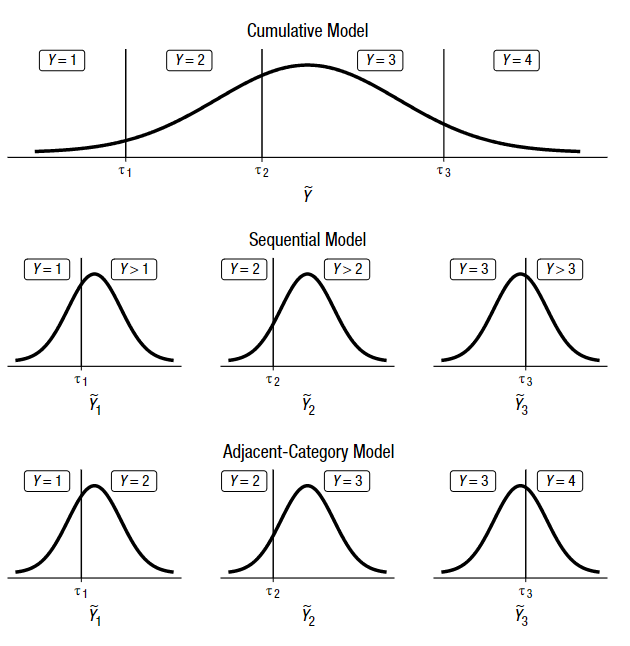
\includegraphics[width=1\linewidth]{img/fig-ordinal-models} 

}

\caption{Cumulative model. Adapted from Bürkner and Vuorre (2019).}\label{fig:fig-ordinal-models}
\end{figure}

\normalsize

\subsection{Model notation}\label{model-notation}

In this section we introduce some notation for the CM that is used through the paper and in the R code. We proposed a notation as consistent as possible with the literature and the \texttt{ordinal} R package used in the tutorial. We define \(Y_k\) as the observed ordinal response with \(1, \dots, k\) levels and \(Y^\star\) is the underlying latent variable. The latent variable is segmented using \(k - 1\) thresholds \(\alpha_1, \dots, \alpha_{k - 1}\). Similarly to the generalized linear models framework, we define \(g(x) = \eta\) as the link function that maps probabilities into the linear predictor \(\eta\). To transform back \(\eta\) into probabilities we use the inverse of the link function \(x = g^{-1}(\eta)\). The specific link function define the type of model and require a different R function. For example, when assuming a Gaussian distribution we are fitting a model with a \texttt{probit} link function is the cumulative distribution function \(g(x) = \Phi^{-1}(x) = \eta\) and the inverse of the link function is the inverse cumulative distribution function (or quantile function) defined \(x = g^{-1}(\eta) = \Phi(\eta)\). When modelling an ordinal variable in a cumulative link model we actually modelling the cumulative probability \(P(Y \leq k), k = 1, \dots, k - 1\)\footnote{As done by Agresti (2010), when referring to \(P(Y \leq k)\) we are implicitly conditioning on a particular \(x\) value \(P(Y \leq k | x_i)\)}. Equation \eqref{eq:prob-cum-model1} depict the general cumulative model including predictors \(\mathbf{X}\) and regression coefficients \(\boldsymbol{\beta}\). The minus sign in \(\mathbf{X} \boldsymbol{\beta}\) is used to interpret the \(\beta\) as in the standard regression model (Agresti, 2010) where higher \(\beta\) values corresponds to increased probability of responding higher \(k\) categories.

\begin{equation} 
P(Y \leq k) = g^{-1}(\alpha_k - \mathbf{X} \boldsymbol{\beta}), \;\;k = 1, \dots, k - 1
\label{eq:prob-cum-model1}
\end{equation}

The \(\mathbf{X} \boldsymbol{\beta}\) is the linear predictor \(\eta\) that is the cumulative probability \(P(Y \leq k)\) transformed using the link function \(g()\). To obtain the probability of a single outcome \(P(Y = k)\) we can compute the difference between cumulative probabilities as shown in Equation \eqref{eq:eq:prob-cum-model2}.

\begin{equation} 
P(Y = k) = g^{-1}(\alpha_k - \eta) -  g^{-1}(\alpha_{k - 1} - \eta), \;\;k = 1, \dots, k - 1
\label{eq:prob-cum-model2}
\end{equation}

There are always two special cases when computing the probability of a single outcome \(Y\) that is when \(Y = 1\) and \(Y = k\). In the first case the cumulative probability is calculated from \(-\infty\) that is the same as temporary assuming an \(\alpha_0 = -\infty\). In the second case (\(Y = 1\)) the probability is calculated as \(P(Y = k) = 1 - g^{-1}(\alpha_{k - 1} - \eta)\) that is the same as assuming a temporary threshold \(\alpha_k = +\infty\). The Figure \ref{fig:fig-explain-cumulative} shows how the single probabilities of the ordinal outcome are calculated from cumulative probabilities.

\scriptsize

\begin{figure}

{\centering 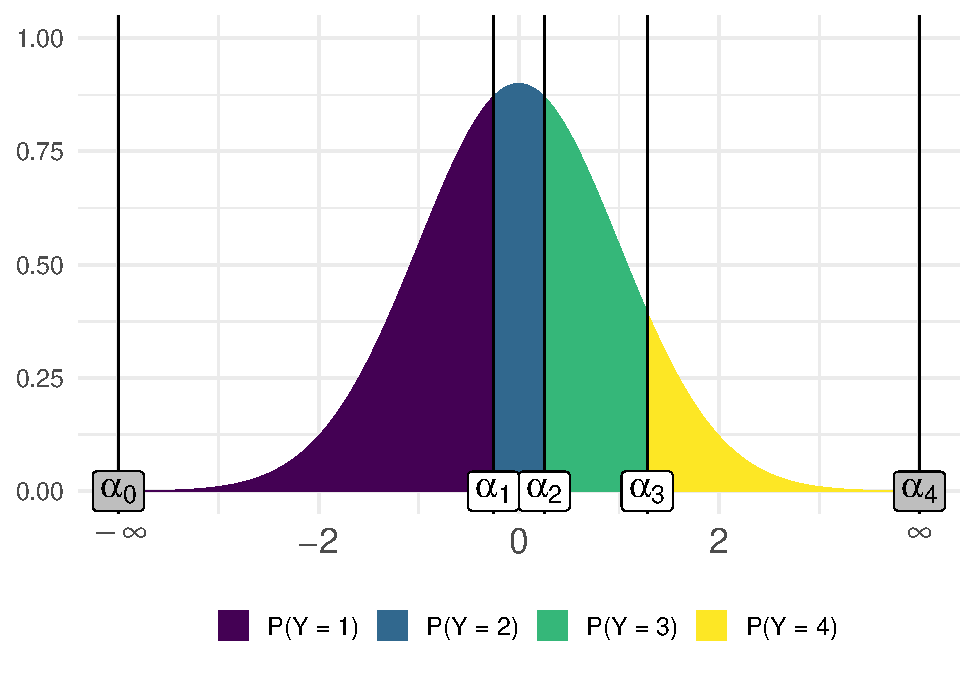
\includegraphics{paper-new_files/figure-latex/fig-explain-cumulative-1} 

}

\caption{caption here}\label{fig:fig-explain-cumulative}
\end{figure}

\normalsize

The same model can be written in the so-called latent formulation as reported in Equation \eqref{eq:latent-model}. The model is no longer directly about the cumulative probabilities but focused on the continuous latent variable \(Y^\star\) as a function of the linear predictor \(\eta = \mathbf{X} \boldsymbol{\beta}\) similar to a standard linear regression.

\begin{equation} 
Y^\star_i = \eta + \epsilon_i
\label{eq:latent-model}
\end{equation}

The crucial part is \(\epsilon_i\) that is the random component of the model coming from a certain probability distribution. For a \emph{probit} model, errors are sampled from a standard Gaussian distribution while for a \emph{logit} model from a standard logistic distribution. Following the notation by Gerhard Tutz (2022), the observed ordinal value \(Y_i = k\) comes from \(Y^\star_i\) belonging to the interval defined by the thresholds \(Y_i = k \iff \alpha_{k - 1} < Y^\star_i < \alpha_{k}\) where \(- \infty = \alpha_0 < \alpha_1 < \dots< \alpha_{k - 1} < \alpha_k = \infty\).

In the basic version of the model, the thresholds \(\alpha_k\) are considered as fixed and being part of the measurement procedure (Liddell \& Kruschke, 2018) and do not vary as a function of the predictors. In a more sophisticated version of the model called location-shift (Gerhard Tutz, 2022), both the location \(\mu\) and the thresholds \(\alpha_k\) can vary as a function of the predictors. Gerhard Tutz (2022) described also another version of the model called location-scale (Cox, 1995; Rigby \& Stasinopoulos, 2005; Gerhard Tutz, 2022) where the location \(\mu\) and the scale \(\sigma^2\) of the distribution can vary as a function of the predictors.

The model can be also formalized in alternative ways. Liddell and Kruschke (2018) and Kruschke (2015) proposed a Bayesian version of the model with a different threshold parametrization. Gelman, Hill, and Vehtari (2020) proposed three alternative parametrizations focusing on different definition of the thresholds.

\subsection{Link function}\label{link-function}

The cumulative link model implemented in Equations \eqref{eq:prob-cum-model1} and \eqref{eq:latent-model} can be considered the general formulation that requires specifying the link function \(g(\cdot)\) or the errors distribution \(\epsilon_i \sim D(\mu, \sigma^2)\). Among several available functions the \emph{logit} and \emph{probit} models are the most common. The \emph{logit} model assume a \emph{logit} link function and a logistic distribution as latent variable. On the other side, the \emph{probit} model assume a Gaussian distribution.

The two models provide similar results with a different parameters interpretation. In the next sections we will illustrate the differences and simulation strategies. Figure \ref{fig:fig-logit-vs-probit} depicts the two distributions while Table \ref{tab:tab-model-summary} summarise the presented cumulative models with the proposed link function and the corresponding R code.

In terms of parameters, both distributions can be defined with a location \(\mu\) and a scale \(s\) parameter. The standard normal distribution has \(\mu = 0\) and \(s = 1\). Furthermore the variance corresponds to the scale \(s^2 = \sigma^2 = 1\). The variance of the logistic distribution is \(\sigma^2 = \frac{s^2\pi^2}{3}\). The standard logistic distribution has \(\mu = 0\) and \(s^2 = 1\) thus the standard deviation simplified to \(\frac{\pi}{\sqrt{3}} \approx 1.81\). In practical terms, fixing \(\mu\) and \(s\) lead to an higher standard deviation for the logistic distribution.

\scriptsize

\begin{figure}

{\centering 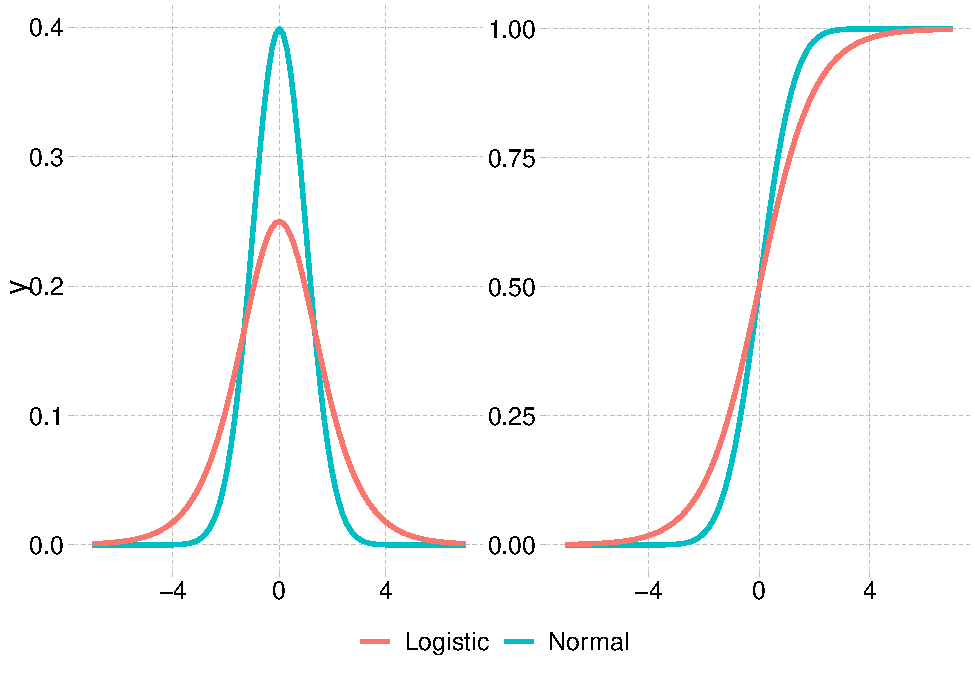
\includegraphics{paper-new_files/figure-latex/fig-logit-vs-probit-1} 

}

\caption{caption here}\label{fig:fig-logit-vs-probit}
\end{figure}

\normalsize

\scriptsize

\begin{table}

\caption{\label{tab:tab-model-summary}caption here}
\centering
\begin{tabular}[t]{lllll}
\toprule
\multicolumn{1}{c}{} & \multicolumn{2}{c}{Link Function} & \multicolumn{2}{c}{Inverse Link Function} \\
\cmidrule(l{3pt}r{3pt}){2-3} \cmidrule(l{3pt}r{3pt}){4-5}
Model & Equation & R Code & Equation & R Code\\
\midrule
Cumulative Logit & $\text{logit}(p) = \text{log}(p / (1-p))$ & `qlogis()` & $e^{\text{logit}(p)} / (1 + e^{\text{logit}(p)})$ & `plogis()`\\
Cumulative Probit & $z = \Phi(p)$ & `qnorm()` & $\Phi^{-1}(z)$ & `pnorm()`\\
\bottomrule
\end{tabular}
\end{table}

\normalsize

\section{Model fitting}\label{model-fitting}

For fitting the cumulative models we used the \texttt{ordinal} package (Christensen, 2019). Despite the presence of other possibilities the \texttt{ordinal} package provide the most complete and intuitive way to implement the ordinal models. The syntax is very similar to standard linear models in R and default functions to calculate predictions, perform model comparison, extract relevant model information are implemented similarly to standard regression modelling.\footnote{For a very complete overview of the ordinal package see Christensen (2019) and the Package documentation \url{https://cran.r-project.org/web/packages/ordinal/ordinal.pdf}}.

The function to fit the model is \texttt{clm()} and the model equation is specified using the R formula syntax \texttt{y\ \textasciitilde{}\ x} where \texttt{y} is the ordinal dependent variable and \texttt{x} is one or more predictors eventually including also the interactions. The package also implements mixed-effects models (see the \texttt{clmm()} function) including random intercepts and slopes but the topic is beyond the scope of the current tutorial.

When fitting the model the crucial arguments are the \texttt{formula}, the \texttt{link} function and the \texttt{data}. More advanced arguments are the \texttt{nominal}, \texttt{scale} and \texttt{threshold}.

\begin{itemize}
\tightlist
\item
  \texttt{formula}: the formula \texttt{y\ \textasciitilde{}\ x} with the dependent variable and predictors.
\item
  \texttt{link}: is the link function. In this tutorial we consider only the \emph{logit} and \emph{probit} link but other link functions are available.
\item
  \texttt{data}: is the dataset where with the variables included in the \texttt{formula}
\item
  \texttt{nominal}: formula with predictors where the proportional odds assumption (See Section ) is relaxed (i.e., partial or non proportional odds)
\item
  \texttt{scale}: formula with predictors for the scale (standard deviation) parameter. This argument allow to fit a scale-location model (see Section ). The main \texttt{formula} argument refers to predictors on the location parameter (i.e., the mean \(\mu\)).
\item
  \texttt{threshold}: different structures for estimating the thresholds. The default is \texttt{threshold\ =\ "flexible"} where \(k - 1\) threshold (where \(k\) is the number of ordinal levels for \(Y\)) are estimated.
\end{itemize}

We can start by fitting a simple model, highlighting the crucial parameters where the detailed explanation will be expanded in the next sections. Table contains simulated data from \(n = 100\) participants rating the agreement about a certain item with \(k = 4\) ordered options. The participants are divided into two groups (predictor \(x\)). We can fit a cumulative link model with \texttt{clm()} function and check the model summary.

\scriptsize

\begin{verbatim}
##   group mean median   sd                  Y1                  Y2
## a     a 2.46      2 1.20 **15** (*p = 0.30*) **11** (*p = 0.22*)
## b     b 3.26      4 0.94  **2** (*p = 0.04*) **11** (*p = 0.22*)
##                    Y3                  Y4
## a **10** (*p = 0.20*) **14** (*p = 0.28*)
## b  **9** (*p = 0.18*) **28** (*p = 0.56*)
\end{verbatim}

\normalsize

\scriptsize

\normalsize

\scriptsize

\begin{verbatim}
## formula: y ~ x
## data:    dat
## 
##  link  threshold nobs logLik  AIC    niter max.grad cond.H 
##  logit flexible  100  -125.31 258.63 5(0)  3.87e-12 2.1e+01
## 
## Coefficients:
##    Estimate Std. Error z value Pr(>|z|)    
## xb   1.3088     0.3828   3.419 0.000629 ***
## ---
## Signif. codes:  0 '***' 0.001 '**' 0.01 '*' 0.05 '.' 0.1 ' ' 1
## 
## Threshold coefficients:
##     Estimate Std. Error z value
## 1|2  -1.0373     0.3074  -3.374
## 2|3   0.1947     0.2791   0.698
## 3|4   1.0282     0.2947   3.489
\end{verbatim}

\normalsize

The two main sections of the model summary are the \emph{Coefficients} section reporting the regression coefficients \(\beta\) and the \emph{Threshold} section reporting the \(\alpha\) estimation. Given that \(k = 4\) we have \(k - 1 = 3\) thresholds and a single \(\beta\) associated with the \(x\) effect. As in standard regression models, when \(x\) is a categorical predictor with \(j\) level, we will estimate \(j - 1\) regression coefficients where the interpretation depends on the contrast coding {[}for an overview about contrasts coding schemes see Schad, Vasishth, Hohenstein, and Kliegl (2020){]}\footnote{In R the default is the dummy coding where a factor of \(j\) levels is converted into \(j - 1\) dummy variables. By default, the first level of the factor is taken as the reference level and the \(j - 1\) coefficients represent the comparison between the other levels and the reference.}

\section{Interpreting parameters}\label{interpreting-parameters}

\subsection{\texorpdfstring{\emph{Logit Model}. Odds and odds ratio}{Logit Model. Odds and odds ratio}}\label{logit-model.-odds-and-odds-ratio}

To understand the logit model we need to introduce odds and odds ratio. The odds of a probability \(p\) is defined as \(\frac{p}{1 - p}\) thus the probability of success divided by the probability of failure. The odds takes value ranging from 0 to \(\infty\). For example with a probability of \(p = 0.8\) we have an odds of \(4\), thus we have a 4 successes for each failure. The same as having \(p = 0.2\) and an odds of \(0.25\) means that for each \(0.25\) successes we have a failure or that we have \(4\) failures for each success. When comparing two groups or conditions we can compare the two odds calculating an odds ratio. The odds ratio is the mostly used statistics to compare groups or conditions on a binary outcome. An odds ratio of \(4\) means that the odds of success at the numerator is 4 times higher than the odds of success at the denominator. The Figure \ref{fig:fig-odds-example} shows the relationship between probabilities and odds. The logit transformation is about taking the logarithm of the odds creating a symmetric function ranging from \(-\infty\) to \(\infty\) with \(p = 0.5\) as the midpoint because \(\text{log}(\frac{0.5}{1 - 0.5}) = 0\). The standard logistic regression with two outcome model the logit transformed probability.

\scriptsize

\begin{figure}

{\centering 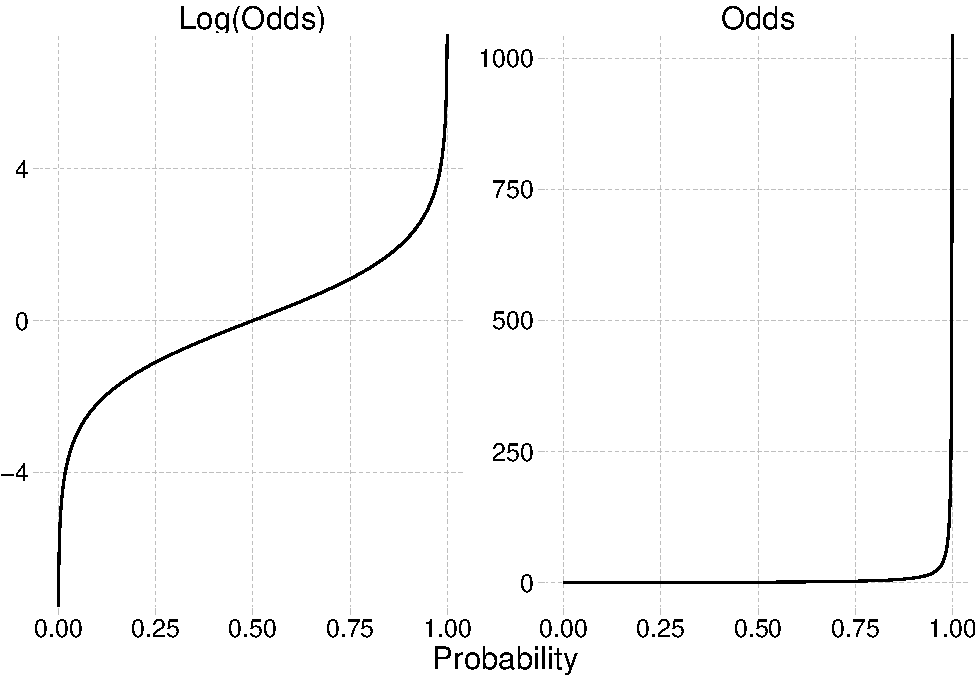
\includegraphics{paper-new_files/figure-latex/fig-odds-example-1} 

}

\caption{(ref:fig-odds-example)}\label{fig:fig-odds-example}
\end{figure}

\normalsize

Odds and odds ratios are clearly defined with \(k = 2\) outcomes. With an ordinal variable and a cumulative model we can use the cumulative odds ratio. With e.g.~\(k = 4\) outcomes we have \(k - 1\) models determined by the cumulative probability in terms of \(P(Y \leq 1), \dots, P(Y \leq k - 1)\). We can manually calculate the odds ratio starting from the previous dataset.

\scriptsize

\begin{Shaded}
\begin{Highlighting}[]
\CommentTok{\# function to calculate odds}
\NormalTok{odds }\OtherTok{\textless{}{-}} \ControlFlowTok{function}\NormalTok{(p) p }\SpecialCharTok{/}\NormalTok{ (}\DecValTok{1} \SpecialCharTok{{-}}\NormalTok{ p)}

\CommentTok{\# probability of Y = 1 for the group a}
\NormalTok{dat}\SpecialCharTok{$}\NormalTok{yn }\OtherTok{\textless{}{-}} \FunctionTok{as.integer}\NormalTok{(dat}\SpecialCharTok{$}\NormalTok{y) }\CommentTok{\# better as number here}
\NormalTok{(p1a }\OtherTok{\textless{}{-}} \FunctionTok{mean}\NormalTok{(dat}\SpecialCharTok{$}\NormalTok{yn[dat}\SpecialCharTok{$}\NormalTok{x }\SpecialCharTok{==} \StringTok{"a"}\NormalTok{] }\SpecialCharTok{==} \DecValTok{1}\NormalTok{))}
\DocumentationTok{\#\# [1] 0.3}

\CommentTok{\# thus P(Y \textgreater{} 1) = 1 {-} p1a}
\FunctionTok{odds}\NormalTok{(p1a)}
\DocumentationTok{\#\# [1] 0.4285714}

\CommentTok{\# odds ratio Y = 1 a vs b}
\NormalTok{(p1b }\OtherTok{\textless{}{-}} \FunctionTok{mean}\NormalTok{(dat}\SpecialCharTok{$}\NormalTok{yn[dat}\SpecialCharTok{$}\NormalTok{x }\SpecialCharTok{==} \StringTok{"b"}\NormalTok{] }\SpecialCharTok{==} \DecValTok{1}\NormalTok{))}
\DocumentationTok{\#\# [1] 0.04}
\FunctionTok{odds}\NormalTok{(p1a) }\SpecialCharTok{/} \FunctionTok{odds}\NormalTok{(p1b)}
\DocumentationTok{\#\# [1] 10.28571}
\end{Highlighting}
\end{Shaded}

\normalsize

For example the probability of responding \(Y = 1\) in the group ``a'' is 0.30 corresponding to an odds of 0.43. When calculating the odds ratio comparing ``a'' vs ``b'' for \(Y = 1\) we obtain that the group ``a'' has 10.29 times the odds of responding \(Y = 1\) compared to the group ``b''.

For an ordinal variable we have \(k\) levels and we can calculate \(k - 1\) cumulative probabilities (excluding the last associated with \(p = 1\)). Thus we have \(k - 1\) odds ratio or what is called a cumulative odds ratio. Basically we repeat the previous steps but on the cumulative probability \(P(Y \leq k), k = 1, \dots, k - 1\). The three odds ratios are very similar correspond to the model estimate \(e^\beta_1\), in R \texttt{exp(fit\$beta)} 3.70. In fact, the logit model essentially estimate the cumulative odds ratio.

\scriptsize

\begin{Shaded}
\begin{Highlighting}[]
\CommentTok{\# the dummy\_ord() is a custom function creating k {-} 1 dummy variable for the cumulative probabilities}

\CommentTok{\# data.frame with the group (x) and the k {-} 1 dummy variables}
\NormalTok{cum\_p }\OtherTok{\textless{}{-}} \FunctionTok{cbind}\NormalTok{(}\AttributeTok{x =}\NormalTok{ dat}\SpecialCharTok{$}\NormalTok{x, }\FunctionTok{dummy\_ord}\NormalTok{(dat}\SpecialCharTok{$}\NormalTok{y))}

\CommentTok{\# calculating the cumulative probability for k {-} 1 variables. }
\CommentTok{\# Taking the average of a series of 0{-}1 is the same as computing the proportion of 1s.}
\NormalTok{(group\_a }\OtherTok{\textless{}{-}} \FunctionTok{apply}\NormalTok{(cum\_p[cum\_p}\SpecialCharTok{$}\NormalTok{x }\SpecialCharTok{==} \StringTok{"a"}\NormalTok{, }\SpecialCharTok{{-}}\DecValTok{1}\NormalTok{], }\DecValTok{2}\NormalTok{, mean))}
\DocumentationTok{\#\# y1vs234 y12vs34 y123vs4 }
\DocumentationTok{\#\#    0.30    0.52    0.72}
\NormalTok{(group\_b }\OtherTok{\textless{}{-}} \FunctionTok{apply}\NormalTok{(cum\_p[cum\_p}\SpecialCharTok{$}\NormalTok{x }\SpecialCharTok{==} \StringTok{"b"}\NormalTok{, }\SpecialCharTok{{-}}\DecValTok{1}\NormalTok{], }\DecValTok{2}\NormalTok{, mean))}
\DocumentationTok{\#\# y1vs234 y12vs34 y123vs4 }
\DocumentationTok{\#\#    0.04    0.26    0.44}

\CommentTok{\# calculating k {-} 1 odds ratios on the cumulative probabilities as a/b}
\FunctionTok{odds}\NormalTok{(group\_a) }\SpecialCharTok{/} \FunctionTok{odds}\NormalTok{(group\_b)}
\DocumentationTok{\#\#   y1vs234   y12vs34   y123vs4 }
\DocumentationTok{\#\# 10.285714  3.083333  3.272727}
\end{Highlighting}
\end{Shaded}

\normalsize

\subsection{Proportional odds assumption}\label{proportional-odds-assumption}

From the previous example, we noticed that the \(k - 1\) odds ratios are very similar (the similarity increase if \(n\) increase). This is not a coincidence but an implicit (until now) assumption made by the CM called \emph{proportional odds} (POA). Following again the taxonomy by Gerhard Tutz (2022), each of the presented ordinal regression model has a basic version making the (POA). There are more advanced versions of the model relaxing this assumption completely (\emph{non proportional odds}) and partially (\emph{partial proportional odds}). The proportional odds assumption is a crucial point when interpreting model parameters. Can be formalized as in Equation ().

Basically if we use the \emph{logit} link function \(g()\) the \(\beta\)s are interpreted as standard odds ratio in the logistic regression. Given that we have \(k > 2\) alternatives there is the need of \(k - 1\) equations. The POA is formalized in Equation \eqref{eq:prop-odds}. Basically the cumulative log odds ratio comparing \(P(Y_k|x_0)\) with \(P(Y_k|x_1)\) is the same regardless the specific \(k\) or threshold \(\alpha\).

The proportional odds is assuming that the regression coefficients \(\beta\) are independent from the thresholds \(\alpha\) thus the effect is the same regardless of the \(Y\) level. Thus \(\beta_1 = \beta_2 \dots = \beta_{k - 1}\). The Figure (\ref{fig:fig-prop-odds}) depicts the proportional odds assumption for the \(k - 1\) logistic curves both for probabilities and linear predictors \(\eta\).

\begin{equation}
\text{logit} (\frac{P(Y \leq 1 |x_1)}{P(Y \leq 1 |x_0)}) = \dots = \text{logit} (\frac{P(Y \leq k - 1 |x_1)}{P(Y \leq k -1 |x_0)})
\label{eq:prop-odds}
\end{equation}

\scriptsize

\begin{figure}

{\centering 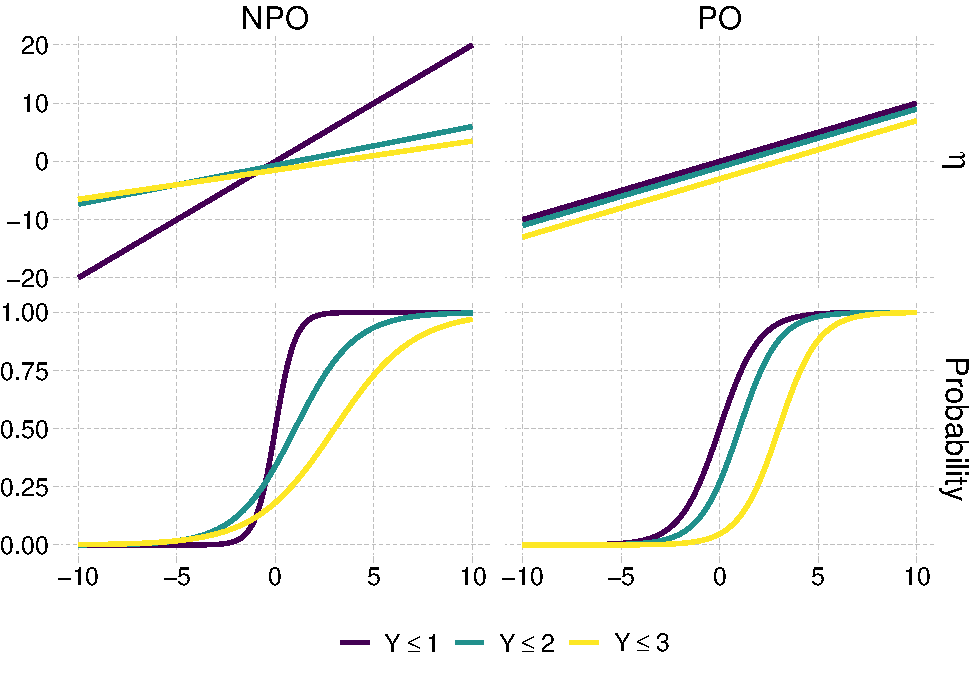
\includegraphics{paper-new_files/figure-latex/fig-prop-odds-1} 

}

\caption{caption here}\label{fig:fig-prop-odds}
\end{figure}

\normalsize

The proportional odds assumption is convenient because regardless of \(k\), the \(\beta_j\) (\(j\) being the number of regression coefficients) effect is assumed to be the same. The model is more parsimonious compared to estimating \(k - 1\) coefficients for each \(\beta_j\) as in the multinomial regression or the non-proportional model.

Given the relatively strong assumption, there are several methods for testing if data are supporting the POA (see Liu, He, Tu, \& Tang, 2023 for an overview). Gerhard Tutz and Berger (2020) suggested a trade-off between assuming/relaxing the POA in terms of implementing \emph{location-shift} or \emph{location-scale} models. Basically these methods should guarantee more flexibility in modelling the observed probabilities reducing the number of parameters. However, these methods and models are outside the scope of the tutorial. In the next section, we provide more details only about the \emph{location-scale} model in terms of parameters interpretation and data simulation.

This can be shown by fitting the model with \texttt{clm()} that by default assume the POA and using the predicted probabilities to compute the odds ratios. In the following code we computed the odds ratio comparing \(x_a\) and \(x_b\) when \(k \leq 1\) and \(k \leq 2\).

\scriptsize

\begin{Shaded}
\begin{Highlighting}[]
\CommentTok{\# fitting the model}
\NormalTok{fit }\OtherTok{\textless{}{-}} \FunctionTok{clm}\NormalTok{(y }\SpecialCharTok{\textasciitilde{}}\NormalTok{ x, }\AttributeTok{data =}\NormalTok{ dat, }\AttributeTok{link =} \StringTok{"logit"}\NormalTok{)}

\CommentTok{\# extracting the predicted probabilities for the two groups}
\NormalTok{pr }\OtherTok{\textless{}{-}} \FunctionTok{predict}\NormalTok{(fit, }\FunctionTok{data.frame}\NormalTok{(}\AttributeTok{x =} \FunctionTok{unique}\NormalTok{(x)))}\SpecialCharTok{$}\NormalTok{fit}

\CommentTok{\# y \textless{}= 1}
\NormalTok{y1a }\OtherTok{\textless{}{-}}\NormalTok{ pr[}\DecValTok{1}\NormalTok{, }\DecValTok{1}\NormalTok{]}
\NormalTok{y1b }\OtherTok{\textless{}{-}}\NormalTok{ pr[}\DecValTok{2}\NormalTok{, }\DecValTok{1}\NormalTok{]}

\CommentTok{\# y \textless{}= 2}
\NormalTok{y12a }\OtherTok{\textless{}{-}} \FunctionTok{sum}\NormalTok{(pr[}\DecValTok{1}\NormalTok{, }\DecValTok{1}\SpecialCharTok{:}\DecValTok{2}\NormalTok{])}
\NormalTok{y12b }\OtherTok{\textless{}{-}} \FunctionTok{sum}\NormalTok{(pr[}\DecValTok{2}\NormalTok{, }\DecValTok{1}\SpecialCharTok{:}\DecValTok{2}\NormalTok{])}

\CommentTok{\# odds ratio y \textless{}= 1 (a vs b) VS y \textless{}= 2 (a vs b)}
\FunctionTok{odds}\NormalTok{(y1a) }\SpecialCharTok{/} \FunctionTok{odds}\NormalTok{(y1b)}
\DocumentationTok{\#\# [1] 3.701591}
\FunctionTok{odds}\NormalTok{(y12a) }\SpecialCharTok{/} \FunctionTok{odds}\NormalTok{(y12b)}
\DocumentationTok{\#\# [1] 3.701591}
\end{Highlighting}
\end{Shaded}

\normalsize

In this case the odds ratio is exactly the same because the model (thus the predicted probabilities) assume the POA. When estimating the \(k - 1\) odds ratio from the data results could be different. In fact, the discrepancy between the odds ratio is an index of POA violation. metti qualche riferimento, magari a supplementary.

\subsubsection{\texorpdfstring{Proportional odds and \emph{probit} model}{Proportional odds and probit model}}\label{proportional-odds-and-probit-model}

The proportional odds assumption is relevant only for the \emph{logit} model because of the link function that put \(\beta\) as log odds. However the concept of the proportional odds that is more generally called parallel slopes assumption is assumed also for the probit model. Equation \eqref{eq:probit-prop-odds} depict the parallel slopes assumption for a probit model. Basically the difference in \(z\) for a unit increase in \(x\) (i.e., the slope) is the same regardless the \(Y\) level. This can be directly demonstrated in the same way as for the logit model. We use the same dataset presented in Table \ref{tab:tab-prop-ord-ex} but fitting a probit model. The difference between the \(z\) scores comparing the two groups calculated on the cumulative probability is the same regardless the \(k - 1\) level.

\[
z_{x_1 - x_0} = \Phi(P \leq k|x_0) - \Phi(P \leq k|x_1) = \dots = \Phi(P \leq k - 1|x_0) - \Phi(P \leq k - 1|x_1)
\]

\scriptsize

\begin{Shaded}
\begin{Highlighting}[]
\CommentTok{\# fitting the model}
\NormalTok{fit }\OtherTok{\textless{}{-}} \FunctionTok{clm}\NormalTok{(y }\SpecialCharTok{\textasciitilde{}}\NormalTok{ x, }\AttributeTok{data =}\NormalTok{ dat, }\AttributeTok{link =} \StringTok{"probit"}\NormalTok{)}

\CommentTok{\# extracting the predicted probabilities for the two groups}
\NormalTok{pr }\OtherTok{\textless{}{-}} \FunctionTok{predict}\NormalTok{(fit, }\FunctionTok{data.frame}\NormalTok{(}\AttributeTok{x =} \FunctionTok{unique}\NormalTok{(x)))}\SpecialCharTok{$}\NormalTok{fit}

\CommentTok{\# y \textless{}= 1}
\NormalTok{y1a }\OtherTok{\textless{}{-}}\NormalTok{ pr[}\DecValTok{1}\NormalTok{, }\DecValTok{1}\NormalTok{]}
\NormalTok{y1b }\OtherTok{\textless{}{-}}\NormalTok{ pr[}\DecValTok{2}\NormalTok{, }\DecValTok{1}\NormalTok{]}

\CommentTok{\# y \textless{}= 2}
\NormalTok{y12a }\OtherTok{\textless{}{-}} \FunctionTok{sum}\NormalTok{(pr[}\DecValTok{1}\NormalTok{, }\DecValTok{1}\SpecialCharTok{:}\DecValTok{2}\NormalTok{])}
\NormalTok{y12b }\OtherTok{\textless{}{-}} \FunctionTok{sum}\NormalTok{(pr[}\DecValTok{2}\NormalTok{, }\DecValTok{1}\SpecialCharTok{:}\DecValTok{2}\NormalTok{])}

\CommentTok{\# z score difference y \textless{}= 1 (a vs b) VS y \textless{}= 2 (a vs b)}
\FunctionTok{qnorm}\NormalTok{(y1a) }\SpecialCharTok{{-}} \FunctionTok{qnorm}\NormalTok{(y1b)}
\DocumentationTok{\#\# [1] 0.8261077}
\FunctionTok{qnorm}\NormalTok{(y12a) }\SpecialCharTok{{-}} \FunctionTok{qnorm}\NormalTok{(y12b)}
\DocumentationTok{\#\# [1] 0.8261077}
\end{Highlighting}
\end{Shaded}

\normalsize

\subsection{\texorpdfstring{\emph{Probit Model} \(z\) scores}{Probit Model z scores}}\label{probit-model-z-scores}

The alternative to fitting a cumulative logit model is using a standard normal distribution thus fitting a \emph{probit} model. The main difference is that the latent distribution is now a Gaussian distribution with \(\mu = 0\) and \(\sigma^2 = 1\) and the link function is the cumulative Gaussian distribution function \(\Phi\) implemented in R with the \texttt{pnorm()} function. The inverse of the Gaussian cumulative distribution function is \(\Phi^{-1}\) implemented in R with the \texttt{qnorm()} function. The logistic and normal distribution are very similar, with the logistic having more variance.

The main difference regards the parameters interpretation. In the logit model the \(\beta\) are the log odds ratio. For categorical variables they represents the increase in the log odds of moving from one level to the other while for numerical variables is the increase in the log odds for a unit increase in \(x\). For the probit model, the \(\beta\) is the increase in terms of \(z\) scores for a unit increase in \(x\). This is very convenient especially for categorical variables because parameters can be intepreted as a Cohen's \(d\) like measure. Thinking about the latent distributions, the \(\beta\) is the shift in the latent mean comparing two or more groups or the slope of latent scores as a function of a numeric \(x\). The intepretation in terms of shifting the latent mean holds also for the logistic model. However, the standard deviation of the standard logistic regression is \(\frac{\pi}{\sqrt{3}} \approx 1.81\)\footnote{Actually the variance of the logistic distribution is \(\frac{s^2\pi^2}{3}\) and the standard deviation \(\frac{s\pi}{\sqrt{3}}\) where \(s\) is the scale of the distribution. For the standard logistic distribution \(s = 1\) (as for the standard normal distribution). For the standard normal distribution \(s^2 = \sigma^2 = 1\)}. The \(\beta\) for the logistic distribution can be interpreted as the location shift of the latent logistic distribution by \(\frac{\pi}{\sqrt{3}}\) standard deviations.

Another advantage of the probit model is the possibility to directly map parameters from signal detection theory (Green, Swets, \& Others, 1966; Stanislaw \& Todorov, 1999) into the model coefficients. In practical terms, the thresholds \(\alpha\) are the criterion cut-offs and the \(\beta_1\) is the d\('\) parameter (DeCarlo, 1998; Knoblauch \& Maloney, 2012).

qualcosa in più qui

\subsection{Simulating data}\label{simulating-data}

There are mainly two ways to simulate data. The first method concerns simulating starting from the latent formulation of the ordinal model. Basically we can simulate the underlying latent distribution and then fixing the thresholds converting the latent continuous variable into the observed ordinal variable.

\subsubsection{Simulating from a multinomial distribution}\label{simulating-from-a-multinomial-distribution}

The first method to simulate ordinal data as a function of predictors is by calculating the true probabilities \(g^{-1}(\eta)\) as a function of predictors and then sample from a multinomial distribution\footnote{In R we are using the \texttt{sample()} function that simulate values from a \emph{categorical} distribution. The \emph{categorical} distribution is considered a special case of the multinomial distribution}. This is similar to the general method to simulate data for a generalized linear model where the linear predictors \(\eta\) are calculated and data are generated from the corresponding probability distribution of the random component. The following code box simulate a \(n\) binary trials with a continuous predictor \(x\).

\scriptsize

\begin{figure}

{\centering 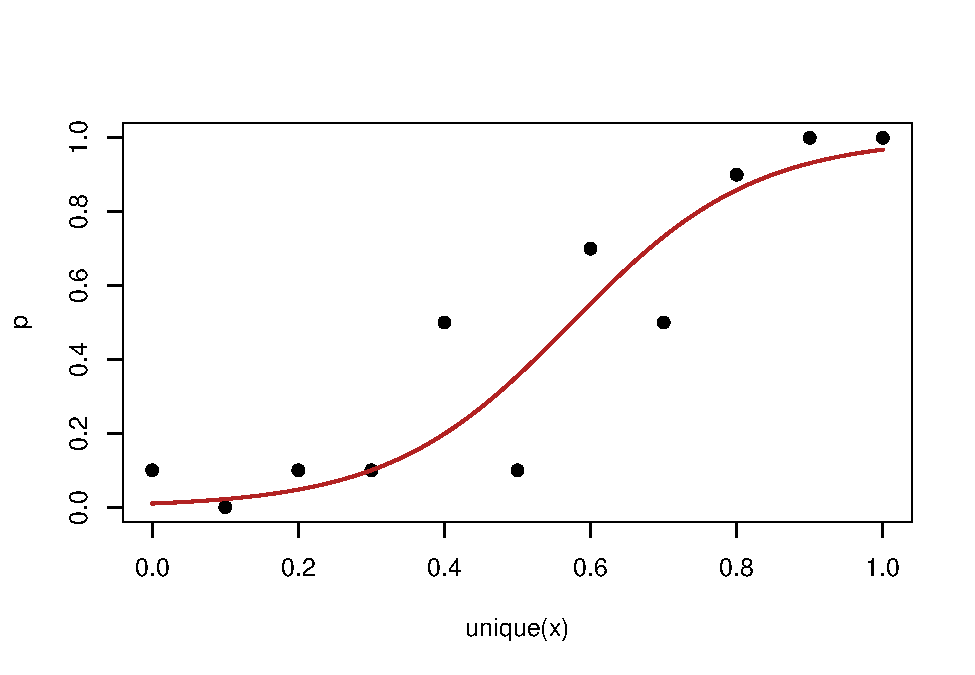
\includegraphics{paper-new_files/figure-latex/unnamed-chunk-6-1} 

}

\caption{ }\label{fig:unnamed-chunk-6}
\end{figure}

\normalsize

Essentially the \texttt{lp} (\(\eta_i\)) vector contains true probability of success (\(p_i|x_i = g^{-1}(\eta_i)\)) for the \(x_i\) level of the predictor. Then to introduce the random part of the model, we can use \(p_i\) to generate binary values from a Binomial (in this specific case a Bernoulli) distribution. This create \texttt{y} that is the vector of 0-1 values generated using the true probabilities of success. The supplementary materials contains a more extensive example for simulating data for generalized linear models.

We can apply the same idea to an ordinal outcome but we need \(k - 1\) equations (compared to the previous example) where \(k\) is the number of ordinal levels. Let's simulate a similar design with a continuous \(x\) predictor and \(k = 4\) options. We fix the baseline probabilities where \(x = 0\) as uniform thus \(p(y_1) = p(y_2) = ... p(y_k) = 1/k\). The proposed workflow for the simulation is:

\begin{enumerate}
\def\labelenumi{\arabic{enumi}.}
\tightlist
\item
  Define \(n\) (number of observations) and \(k\) (number of ordinal outcomes)
\item
  Define the regression coefficients \(\beta\)s.
\item
  Define the baseline probabilities when \(x = 0\). These probabilities can be converted to the corresponding thresholds \(\alpha\) choosing the appropriate link function (\emph{logit} or \emph{probit}).
\item
  Calculate the linear predictors \(\eta\) using \(k - 1\) equations combining the predictors \(\mathbf{X}\) and regression coefficients \(\boldsymbol{\beta}\).
\item
  Apply the inverse of the link function \(g^{-1}(\eta)\) on the linear predictor and calculate the cumulative probabilities \(p(y \leq 1|x), p(y \leq 2|x), ... p(y \leq k - 1|x)\).
\item
  Calculate for each observation the probability of the \(k\) outcome as the difference between cumulative probabilities. For example, the probability of \(P(y = 2) = P(y \leq 2) - P(y \leq 1)\). This is implemented in R by adding a columns of zeros and ones respectively at the beginning and end of the matrix of cumulative probabilities because the probability of the first \(Y = 1\) level is the cumulative probability from \(- \infty\) to the first threshold and the probability of \(Y = k\) is obtained removing \(P(Y \leq k - 1)\) from one.
\item
  Sample \(n\) outcomes from a multinomial distribution, choosing between \(k\) alternatives with the calculated probabilities.
\end{enumerate}

\scriptsize

\normalsize

The linear predictors (\(\eta\)) can be seen in the Figure ref. The \(g\) in this case is the cumulative \emph{probit} function \(\Phi\).

\scriptsize

\begin{figure}

{\centering 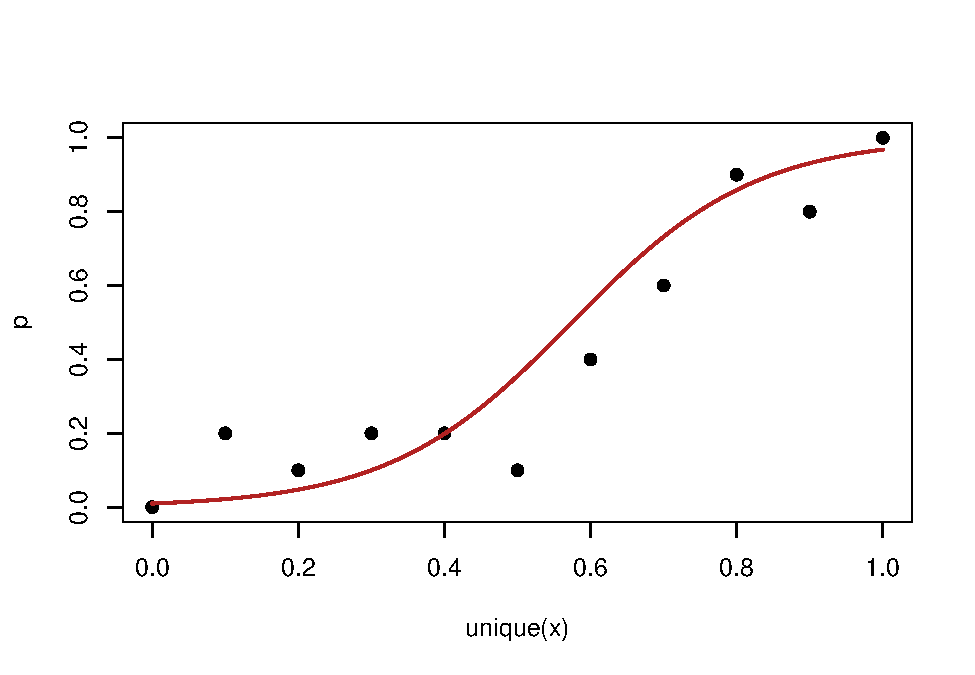
\includegraphics{paper-new_files/figure-latex/unnamed-chunk-8-1} 

}

\caption{ }\label{fig:unnamed-chunk-8}
\end{figure}

\normalsize

Now we can apply the inverse of the link function \(g^{-1} = \Phi^{-1}\) to calculate the corresponding cumulative probabilities.

\scriptsize

\normalsize

\scriptsize

\begin{verbatim}
##    p_y1  p_y2  p_y3  p_y4
## 1 0.409 0.263 0.197 0.131
## 2 0.389 0.264 0.204 0.143
## 3 0.429 0.261 0.189 0.121
## 4 0.119 0.188 0.261 0.433
## 5   ...   ...   ...   ...
## 6 0.147 0.207 0.264 0.383
## 7 0.328 0.263 0.226 0.183
## 8 0.389 0.264 0.204 0.143
## 9 0.488 0.252 0.166 0.094
\end{verbatim}

\normalsize

We can plot the expected effect of \(\beta_1\) on the \(k\) probabilities using the \texttt{num\_latent\_plot()} function (see Figure \ref{fig:sim-with-probs-lat-plot}). Finally we sample using the \texttt{sample()} function using the calculated probabilities.

\scriptsize

\begin{figure}

{\centering 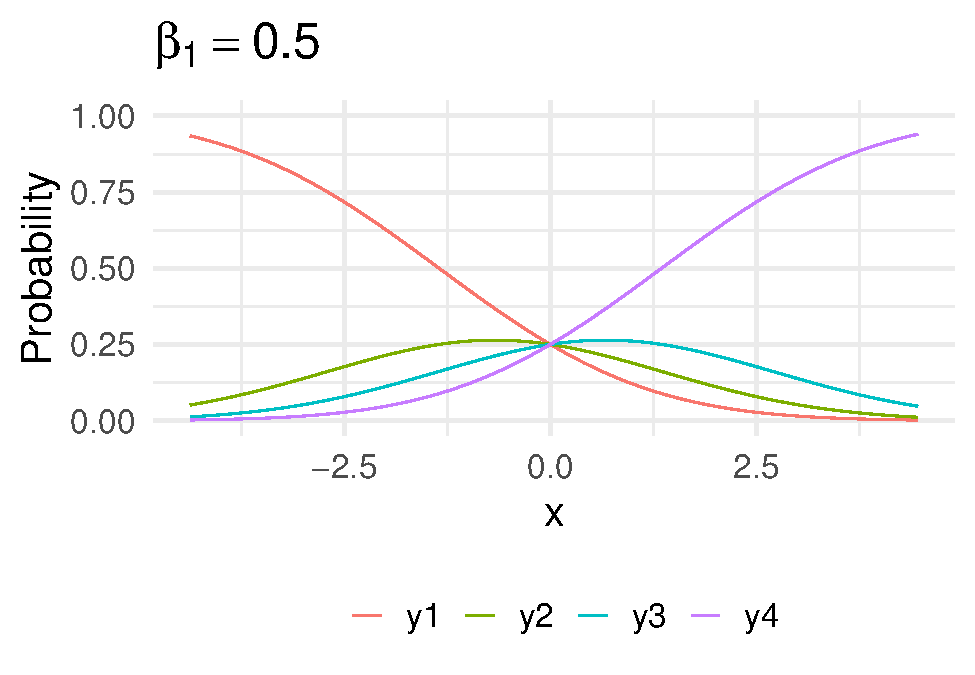
\includegraphics{paper-new_files/figure-latex/sim-with-probs-lat-plot-1} 

}

\caption{sim-with-probs-lat-plot}\label{fig:sim-with-probs-lat-plot}
\end{figure}

\normalsize

\scriptsize

\normalsize

To check the simulation result we can increase the number of observations, fit the model using the \texttt{ordinal::clm()} function and assess the recovery of simulated parameters.

\scriptsize

\normalsize

\scriptsize

\normalsize

\subsubsection{Simulating from the latent distribution}\label{simulating-from-the-latent-distribution}

An equivalent but more efficient way to simulate an ordinal outcome is using the latent formulation of the model. This require simulating a standard linear regression using the appropriate data generation function (\emph{logistic} or \emph{normal}) and the cutting the latent values according to the thresholds \(\alpha\). The workflow is slightly different compared to the previous approach.

\begin{enumerate}
\def\labelenumi{\arabic{enumi}.}
\tightlist
\item
  Define \(n\) (number of observations) and \(k\) (number of ordinal outcomes)
\item
  Define the regression coefficients \(\beta\)
\item
  Define the baseline probabilities when \(x = 0\). These probabilities can be converted to the corresponding thresholds \(\alpha\) choosing the appropriate link function (\emph{logit} or \emph{probit}).
\item
  Calculate the linear predictors \(\eta\) using \(k - 1\) equations combining the predictors \(\mathbf{X}\), the regression coefficients \(\boldsymbol{\beta}\) and the error \(\mathbf{\epsilon}\) sampled from the appropriate probability distribution.
\item
  Cut the latent variable into \(k\) areas using the thresholds \(\alpha\) and assign the corresponding ordinal value. This step simply checks if the latent value \(Y^{\star}_i\) is between two threshold values and assign the corresponding value. This can be done using the \texttt{cut()} or the \texttt{findInterval()} functions.
\end{enumerate}

\scriptsize

\normalsize

The Figure (put crossref) depict the simulated \(Y^{*}\) and the corresponding ordinal value. As for the previous simulation we can fit the model using \texttt{clm()} and check the estimated parameters.

\scriptsize

\begin{figure}

{\centering 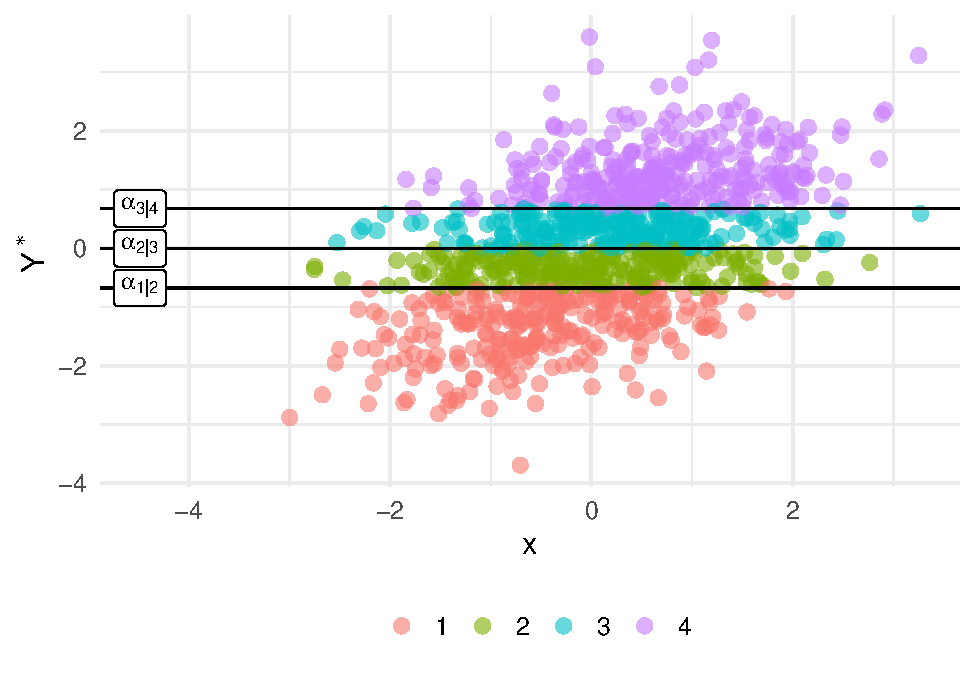
\includegraphics{paper-new_files/figure-latex/unnamed-chunk-14-1} 

}

\caption{ }\label{fig:unnamed-chunk-14}
\end{figure}

\normalsize

\scriptsize

\normalsize

\scriptsize

\normalsize

The simulation using the latent formulation of the model is implemented in the \texttt{sim\_ord\_latent()} function.

\scriptsize

\begin{Shaded}
\begin{Highlighting}[]

\end{Highlighting}
\end{Shaded}

\normalsize

\subsubsection{Choosing parameters values}\label{choosing-parameters-values}

\paragraph{\texorpdfstring{Thresholds \(\alpha\)}{Thresholds \textbackslash alpha}}\label{thresholds-alpha}

The two proposed simulation workflows can be really flexible for simulating complex models with multiple predictors and interactions. The critical part of the simulation is setting appropriate and empirically meaningful parameters values. The thresholds are usually not the crucial part of the statistical inference and model interpretations. In fact, they can be considered as the intercept in standard linear models. In any case to set meaningful \(\alpha\) values the best strategy is to convert them into the corresponding probabilities according to the link function. The thresholds are essentially quantiles of the latent distribution (logistic or normal) without a direct empirical interpretation. The distance between the thresholds determine the probabililty assigned to a specific \(Y\) value. The function \texttt{show\_alpha()} allow to produce a meaningful plot starting from the thresholds or the probabilities. For example, the Figure \ref{fig:fig-show-th-example} depict the threshold/probabilities associated with a four-level ordinal variable.

\scriptsize

\normalsize

\scriptsize

\begin{figure}

{\centering 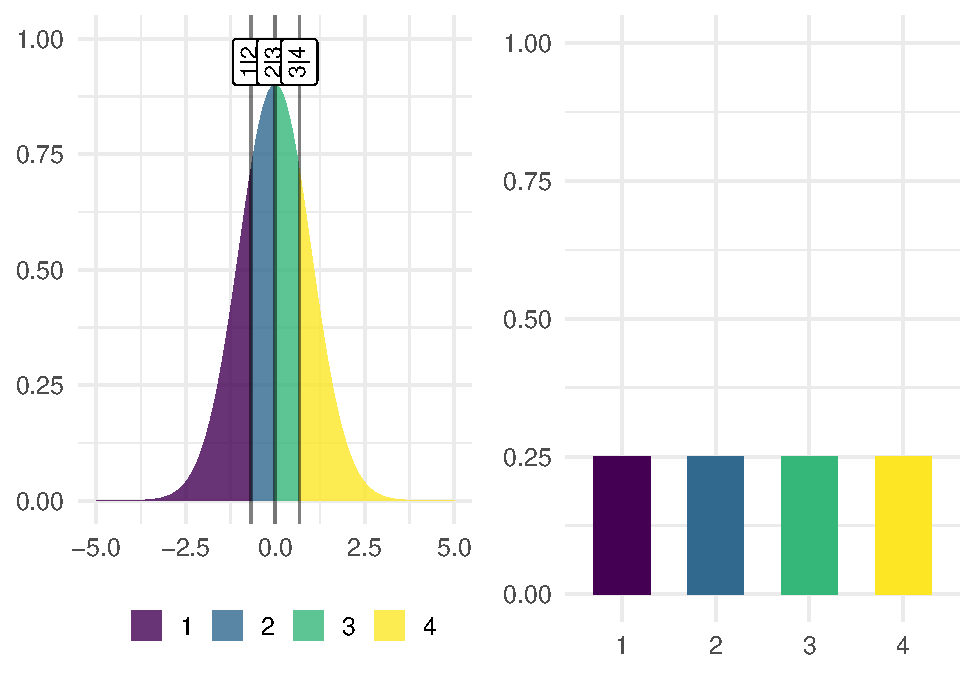
\includegraphics{paper-new_files/figure-latex/fig-show-th-example-1} 

}

\caption{ }\label{fig:fig-show-th-example}
\end{figure}

\normalsize

Thus the thresholds can be fixed according to the desired probabilities distribution. For example, when simulating the difference between two groups on an ordinal variable, the threshold can be set thinking about the response distribution in the reference group. The \texttt{alpha\_to\_prob()} and \texttt{prob\_to\_alpha()} functions can be used to convert between probabilities and thresholds.

\scriptsize

\begin{verbatim}
## [1] -0.2533471  0.0000000  0.8416212
## [1] 0.02275013 0.47724987 0.34134475 0.15865525
\end{verbatim}

\normalsize

\paragraph{\texorpdfstring{Regression coefficients \(\beta\)}{Regression coefficients \textbackslash beta}}\label{regression-coefficients-beta}

As reported in the sections above, the regression coefficients have a different interpretation according to the link function. Fortunately, both parameters have an intuitive interpretation given that they are directly expressed in a interpretable scale. For probit models we can think about standardized mean differences (e.g., Cohen's \(d\)) between categorical variables or standardized regression coefficient for a numerical predictor. For logit models we can fix the parameters thinking about the odds ratios. Meaningful odds ratios can be derived from previous literature, meta-analyses or converting to other effect sizes. For example, Sánchez-Meca, Marín-Martínez, and Chacón-Moscoso (2003) proposed some equations to convert between odds ratios and Cohen's \(d\). Using their approach, a Cohen's \(d\) of 0.5 usually considered a plausible medium effect size corresponds to and odds ratio of \(\approx 2.47\). Another more informative strategy is about plotting the predicted probabilities \(g^{-1}(\eta)\) associated with certain regression coefficients. The \texttt{cat\_latent\_plot()} and \texttt{num\_latent\_plot()} functions can be used to see the impact of choosing a specific regression coefficients for respectively a categorical (Figures \ref{fig:fig-example-cat-latent}) and numerical predictor (Figures \ref{fig:fig-example-num-latent}).

\scriptsize

\begin{Shaded}
\begin{Highlighting}[]
\FunctionTok{cat\_latent\_plot}\NormalTok{(}\AttributeTok{m =} \FunctionTok{c}\NormalTok{(}\DecValTok{0}\NormalTok{, }\FloatTok{0.5}\NormalTok{), }\AttributeTok{s =} \DecValTok{1}\NormalTok{, }\AttributeTok{probs =} \FunctionTok{rep}\NormalTok{(}\DecValTok{1}\SpecialCharTok{/}\DecValTok{4}\NormalTok{, }\DecValTok{4}\NormalTok{), }\AttributeTok{link =} \StringTok{"logit"}\NormalTok{, }\AttributeTok{plot =} \StringTok{"both"}\NormalTok{)}
\end{Highlighting}
\end{Shaded}

\begin{figure}

{\centering 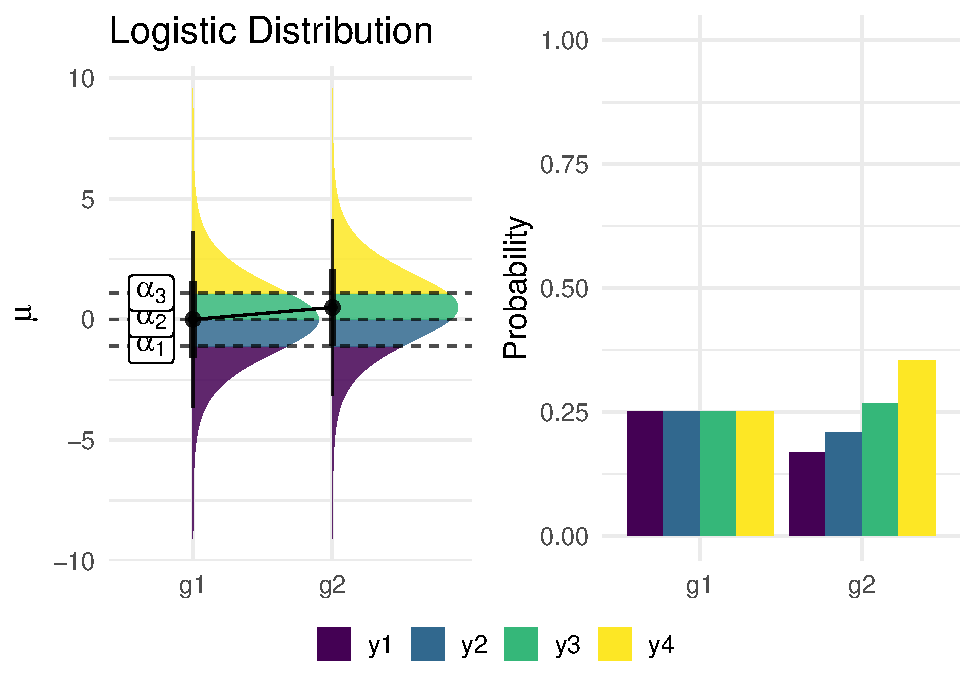
\includegraphics{paper-new_files/figure-latex/fig-example-cat-latent-1} 

}

\caption{caption here}\label{fig:fig-example-cat-latent}
\end{figure}

\normalsize

\scriptsize

\begin{Shaded}
\begin{Highlighting}[]
\FunctionTok{num\_latent\_plot}\NormalTok{(}\AttributeTok{x =} \FunctionTok{runif}\NormalTok{(}\DecValTok{100}\NormalTok{), }\AttributeTok{b1 =} \DecValTok{2}\NormalTok{, }\AttributeTok{probs =} \FunctionTok{c}\NormalTok{(}\FloatTok{0.6}\NormalTok{, }\FloatTok{0.2}\NormalTok{, }\FloatTok{0.1}\NormalTok{, }\FloatTok{0.1}\NormalTok{), }\AttributeTok{link =} \StringTok{"probit"}\NormalTok{)}
\end{Highlighting}
\end{Shaded}

\begin{figure}

{\centering 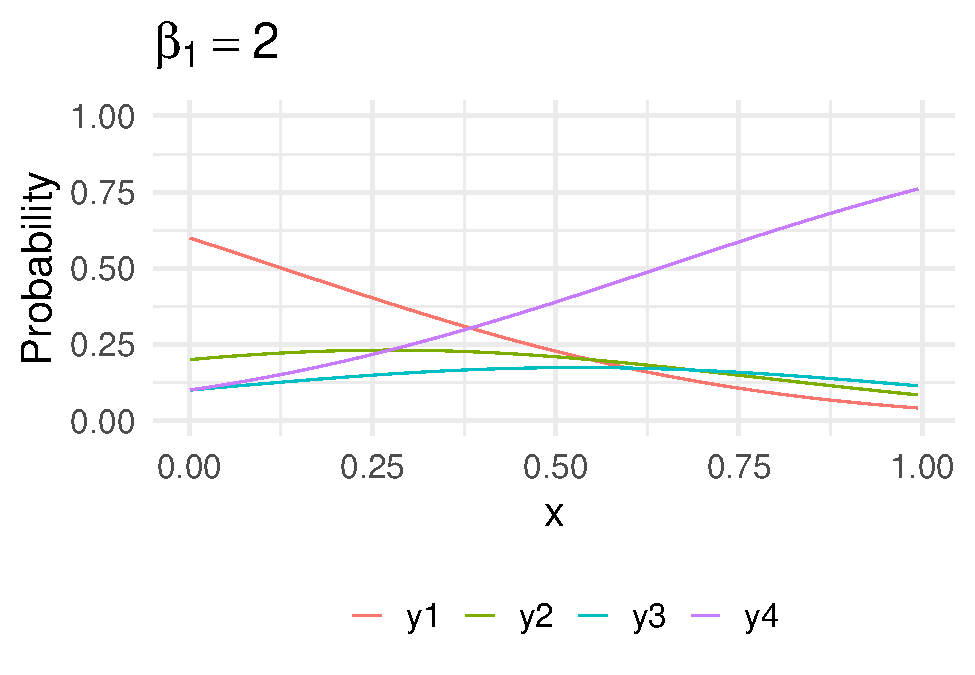
\includegraphics{paper-new_files/figure-latex/fig-example-num-latent-1} 

}

\caption{caption here}\label{fig:fig-example-num-latent}
\end{figure}

\normalsize

\subsection{Scale Effects}\label{scale-effects}

The default ordinal regression model assume that the variance of the underlying latent distribution is the same across condition. This is similar to a standard linear regression assuming the homogeneity of variance. For example, when comparing two groups or conditions we can run a standard linear model (i.e., a t-test) assuming homogeneity of variances or using the Welch t-test (see Delacre, Lakens, \& Leys, 2017). In addition, there are the so-called location-scale models that allows to include predictors also for the scale (e.g., the variance) of the distribution. This can be done also in ordinal regression where instead of assuming the same variance between conditions, the linear predictors can be included. The Equation (number here) expand the previous model including the linear predictor on the scale of the latent distribution.

\begin{equation}
g(P(Y \leq k)) = \frac{\alpha_k - X\beta}{e^{X\zeta}}
\end{equation}

\begin{equation} 
Y^\star_i = \eta + \epsilon_i
\epsilon_i \sim \mathcal{N}(0, e^{X\zeta})
\end{equation}

Where \(X\zeta\) is the linear predictor \(\eta\) for the scale of the distribution. By dafult for both the logit and probit model the scale is fixed to 1. On scale-location models we put predictors on both parameters. Given that the scale cannot be negative we use a log link function \(\eta = \text{log}(X\zeta)\). Figure \ref{fig:example-unequal-variance} depict an example of a comparison between two groups where the two underlying latent distributions have unequal variance. Ignoring the heterogeneity of variances could lead to underestimation of the effect size, reduced power and inflated type-1 error rate (qualche ref qui). Furtermore, as suggested by G. Tutz and Berger (2017) location-scale models can be considered as a more parsimonius approach compared to partially or completely relaxing the proportional odds assumption. Allowing the scale to be different as a function of the predictor create more modelling flexbility. Furthemore, two groups could be theoretically different only in the scale of the latent distribution with a similar location. In this example, the only way to capture group differences is by including a scale effect. The Figure \ref{fig:fig-scale-effect-example} depict the impact of having different scales between two groups on the ordinal probabilities.

Gerhard Tutz (2022) provide a very clear and intuitive explanation of what happen when including a scale effect and how to interpret the result. As suggested before, the scale-location model allow to independently predict changes in the location and the scale. While location shifts are simply interpreted as increasing/decreasing the latent \(\mu\) or the odds of responding a certain category scale effects are not straightforward. As the scale increase (e.g., the variance increase) there is an higher probability mass on extreme categories. On the other side as the scale decrease, responses are more concentrated on single categories. The categories are determined by the location parameter. For example, if one group have a certain latent mean \(\mu_1\) and a small scale \(\sigma^2 = 1/3\) (thus one third compared to the standard version of the distribution), all responses will be focused on categories around the latent mean. On the other side, increasing the scale will increase the cumulative probabilities for all categories and for values that tends to infinity extreme categories are preferred. Clearly, the scale parameter can somehow be interpreted as the response style (concentrated or variable). This is conceptually similar but implemented and interpreted differently to shift-location models {[}Gerhard Tutz (2022); Tutz2020-xq{]} where thresholds are allowed to vary as a function of predictors. Both models tries to increase the flexibility of modelling the probability structure of the responses by adding extra paprameters to predict the probabilities of the ordinal responses.

\scriptsize

\begin{figure}

{\centering 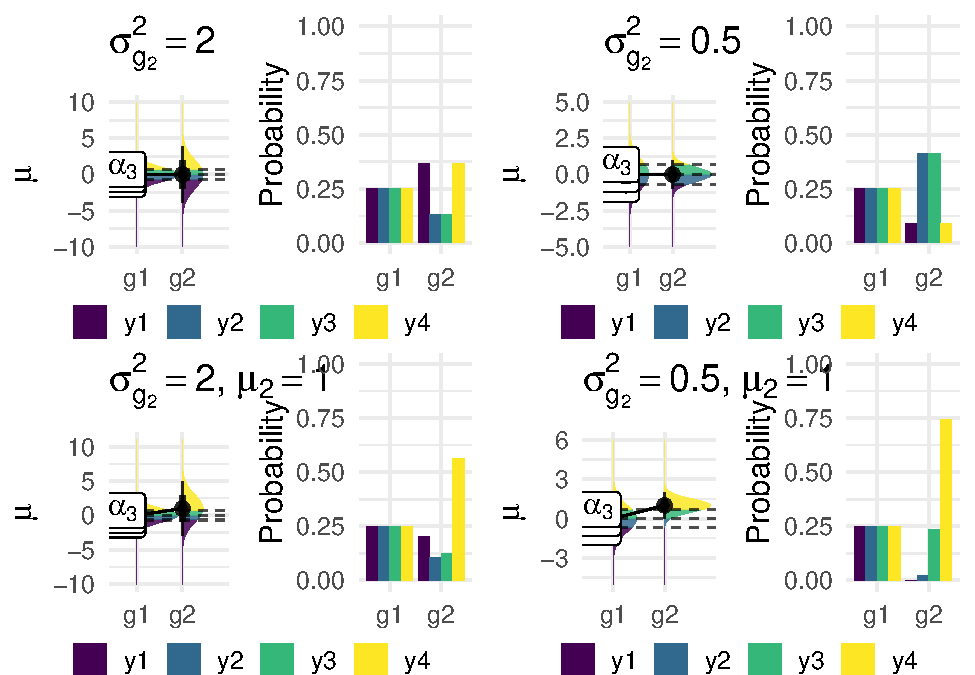
\includegraphics{paper-new_files/figure-latex/unnamed-chunk-19-1} 

}

\caption{ }\label{fig:unnamed-chunk-19}
\end{figure}

\normalsize

\subsubsection{Simulating scale effects}\label{simulating-scale-effects}

The location-scale model can be simulated using the \texttt{sim\_ord\_latent()} function and providing the predictors for the scale parameters. Given the \texttt{log} link function, predictors are provided on the \texttt{log} scale. For example, we simulate the effect of a binary variable \(x\) representing two independent groups predicting the \(k = 5\) response. We simulate a \emph{location} effect of \(\beta_1 = 0.5\) (in \emph{probit} scale) and \(\zeta_1 = \text{log}(2) = 0.70\). The first group has a \(\sigma = 1\) and the second group has \(\sigma = 2\). Again we simulate that the baseline probabilities are uniform for the first group.

\scriptsize

\normalsize

The table (put ref) reports the simulation results.

\scriptsize

\normalsize

To better understand the impact of assuming (or simulating) a different latent scale we fit \(k - 1\) binomial regressions and check the estimated coefficients. We are not simulating a specific beta for each outcome but simulating a scale effect is actually impacting the regression coefficients. When generating data for a binary outcome the linear predictor is composed by \(\eta = \beta_0 + \beta_1x\). The threshold \(\alpha\) and slope of the function can be estimated using \(\alpha = -\frac{\beta_0}{\beta_1}\) and the slope is \(\frac{1}{\beta_1}\) (Faraggi, Izikson, \& Reiser, 2003; Knoblauch \& Maloney, 2012). Under the proportional odds assumption, there is only a change in thresholds \(\alpha\) this a shift in the sigmoid along the \(x\) axis. When including a scale effect a change in the sigmoid is combined with a change in the slope.

\scriptsize

\begin{figure}

{\centering 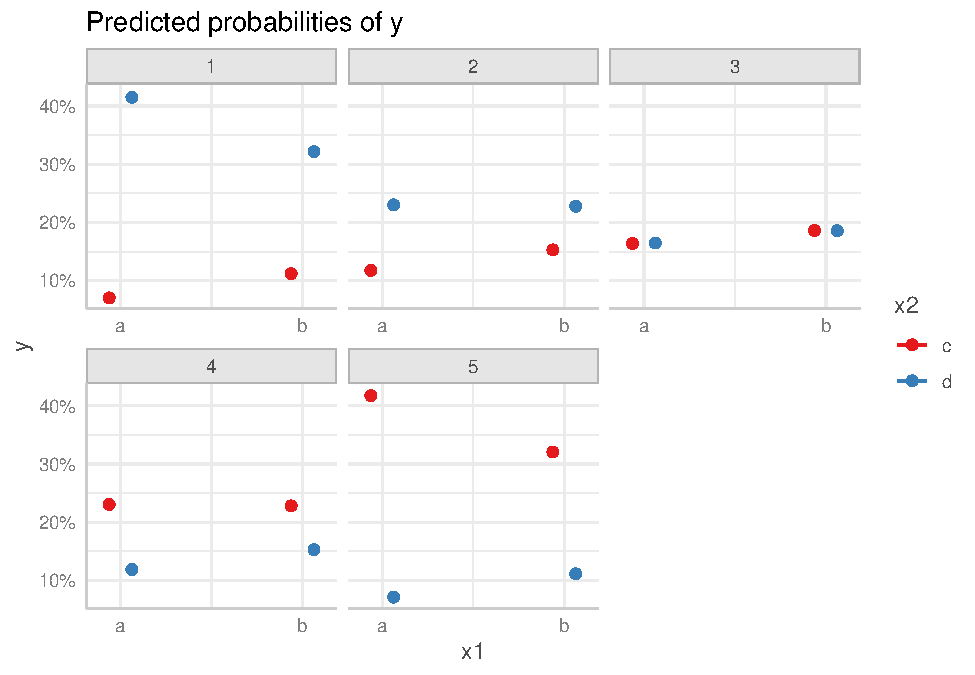
\includegraphics{paper-new_files/figure-latex/unnamed-chunk-22-1} 

}

\caption{ }\label{fig:unnamed-chunk-22}
\end{figure}

\normalsize

\subsection{2x2 interaction}\label{x2-interaction}

A common research design could be a 2x2 factorial design. In this example we have 2 main effects and the interaction. Regardless the link function, we can focus the model equation on the linear predictor. Equation depicts the linear predictor for a 2x2 interaction. With a 2x2 design, a good strategy is to use sum to zero contrasts for the two factors. By default R use dummy coding but here we set the contrasts for \(X_1\) and \(X_2\) as \(0.5\) and \(-0.5\). In this way \(\beta_1\) will be the main effect of \(X_1\), \(\beta_2\) the main effect of \(X_2\) and \(\beta_3\) the interaction (thus the difference of differences).

\[
g(P(Y \leq k))^{-1} = \alpha_k - \beta_1X_{1_i} + \beta_2X_{2_i} + \beta_3X_{1_i}X_{2_i}
\]

\scriptsize

\begin{verbatim}
## formula: y ~ x1 * x2
## data:    dat
## 
##  link   threshold nobs  logLik     AIC        niter max.grad cond.H 
##  probit flexible  4e+05 -597389.03 1194792.06 5(0)  1.42e-07 4.0e+01
## 
## Coefficients:
##         Estimate Std. Error z value Pr(>|z|)    
## x11     0.004798   0.003410   1.407    0.159    
## x21     1.004223   0.003519 285.383   <2e-16 ***
## x11:x21 0.505333   0.006833  73.954   <2e-16 ***
## ---
## Signif. codes:  0 '***' 0.001 '**' 0.01 '*' 0.05 '.' 0.1 ' ' 1
## 
## Threshold coefficients:
##      Estimate Std. Error z value
## 1|2 -0.841241   0.002332  -360.8
## 2|3 -0.254088   0.002092  -121.4
## 3|4  0.250954   0.002092   120.0
## 4|5  0.839533   0.002331   360.2
\end{verbatim}

\normalsize

The parameters intepretation is the same as introduced in the general case. The thresholds \(\alpha\) are fixed the determines the probabilities \(P(Y = k)\) when all predictors are zero. In this case by doing \texttt{alpha\_to\_prob(fit\$alpha,\ link\ =\ "probit")} we should recover the \texttt{bprobs} vector. \texttt{x1} is the main effect thus the difference in \(z\) scores between \emph{a} and \emph{b} averaging over \texttt{x2}. The same holds for \texttt{x2}. \texttt{x1:x2} is the difference of differences in \(z\) scores thus \((ad - ac) - (bd - bc)\).

To visualize the effects there is the \texttt{ggeffect::ggpredict()} function that compute the predictions according to the specified predictors combination. In this case we can plot the interaction using the estimated probability for each group and \(Y\) response.

\scriptsize

\begin{figure}

{\centering 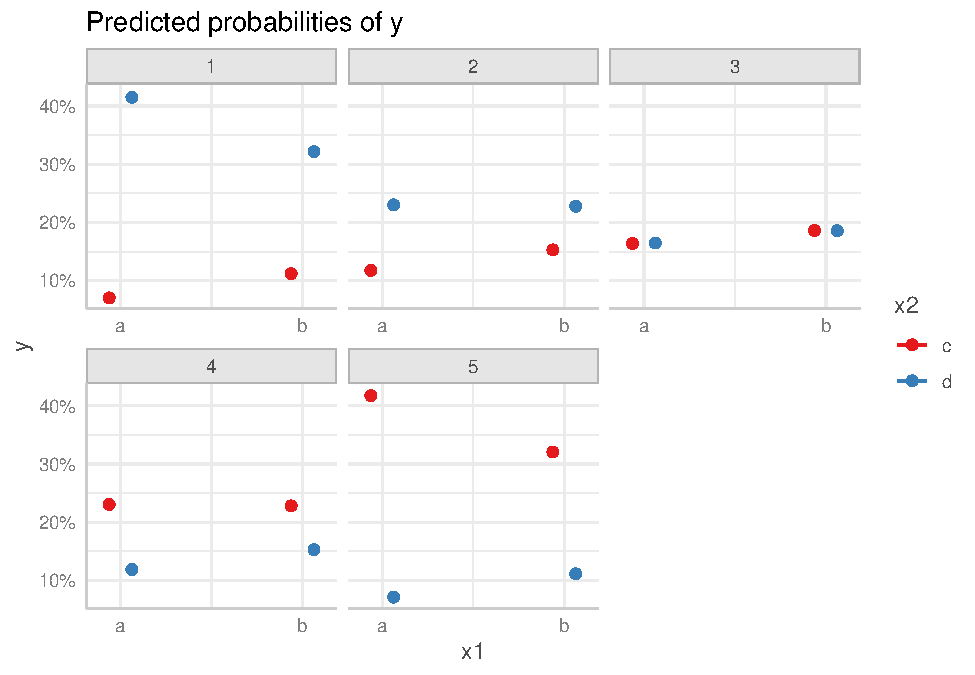
\includegraphics{paper-new_files/figure-latex/unnamed-chunk-24-1} 

}

\caption{ }\label{fig:unnamed-chunk-24}
\end{figure}

\normalsize

\subsection{Numerical by factor interaction}\label{numerical-by-factor-interaction}

Another common scenario is to compute and interaction between a numerical variable \(x\) and a factor \(g\). For simplicity we simulate the factor with two levels and the numerical variable sampled from an uniform distribution \(x \sim \mathcal{U}(0, 1)\). Again, the thresholds \(\alpha\) represents the baseline probabilities when \(x = 0\) and \(g = 0\).

\scriptsize

\begin{verbatim}
## formula: y ~ x * g
## data:    dat
## 
##  link   threshold nobs  logLik     AIC       niter max.grad cond.H 
##  probit flexible  1e+05 -153256.51 306527.02 5(0)  7.97e-08 1.6e+02
## 
## Coefficients:
##      Estimate Std. Error z value Pr(>|z|)    
## x     0.29419    0.01172   25.11   <2e-16 ***
## g1    0.49679    0.01351   36.78   <2e-16 ***
## x:g1  0.51690    0.02343   22.06   <2e-16 ***
## ---
## Signif. codes:  0 '***' 0.001 '**' 0.01 '*' 0.05 '.' 0.1 ' ' 1
## 
## Threshold coefficients:
##      Estimate Std. Error z value
## 1|2 -0.841442   0.007474 -112.59
## 2|3 -0.258062   0.007133  -36.18
## 3|4  0.250592   0.007124   35.18
## 4|5  0.838293   0.007404  113.23
\end{verbatim}

\normalsize

Again, \texttt{x} is the slope of the numerical predictor averaging over \texttt{g} (given that \texttt{g} has been coded with sum to zero contrasts) thus the increase in \(z\) scores for a unit increase in \texttt{x}. \texttt{g1} is the main effect of the factor evaluated when \(x = 0\). To change the interpretation of \texttt{g1} a possibility is to center \texttt{x} differently (e.g., mean centering). The \texttt{x:g1} is the difference in slopes between the two groups.

Regardless of the model complexity, the \texttt{sim\_ord\_latent()} function can be expanded by including more predictors. Clearly, as the model complexity increase, choosing meaningful and empirically plausible parameters became more challenging.

\section{Power Analysis}\label{power-analysis}

In the previous sections we introduced how to simulate standard and scale-location cumulative models and how to fit the corresponding models using the \texttt{clm()} function from the \texttt{ordinal} package. In this section we introduce how to compute the power for some common scenarios. We present an example in a very general form that can be expanded for specific use cases. For example, by simulating a model fixing all effects to zero it is possibile to estimate the type-1 error rate or fixing the sample size and varying the effect size it is possible to do a sensitivity analysis focusing on the smallest effect size of interest (ref qui). The general workflow for a power simulation can be summarized as:

\begin{enumerate}
\def\labelenumi{\arabic{enumi}.}
\tightlist
\item
  Choose the research design, e.g., 2x2 factorial design
\item
  Indentifify the specific effect to focus on. For example the interaction effect, a main effect or a specific contrast
\item
  Write the model equation similarly to what presented in the previous sections and extract the model coefficients
\item
  Choose one of the proposed strategy for simulating data and follows the corresponding steps
\item
  Fit the model and extract the relevant statistics e.g., the p-value of the interaction
\item
  Repeat the simulation a large number of times (e.g, 10000) and store the relevant values from each simulation
\item
  Summarise the simulation results in the appropriate way. For example, the power of the interaction is the number of times the p-value for the interaction test is lower than the critical level divided by the number of simulations.
\end{enumerate}

To make a practical example, we simulate the power of a cumulative link model in detecting an effect of \(d = 0.4\) (probit model) with \(k = 6\) and \(n = 40\) participants per group. We fix the baseline probabilities in the first group as uniform.

descrizione migliore

\scriptsize

\normalsize

Then to compute the power we can simply compute the proportion of p values lower than the critical level. This can be done in R as \texttt{mean(p\ \textless{}=\ alpha)} resulting in an estimated power of 0.39. Clearly using only a single condition is not really informative thus we can vary the sample size across plausible values and check the corresponding power curve.

\scriptsize

\normalsize

\scriptsize

\begin{figure}

{\centering 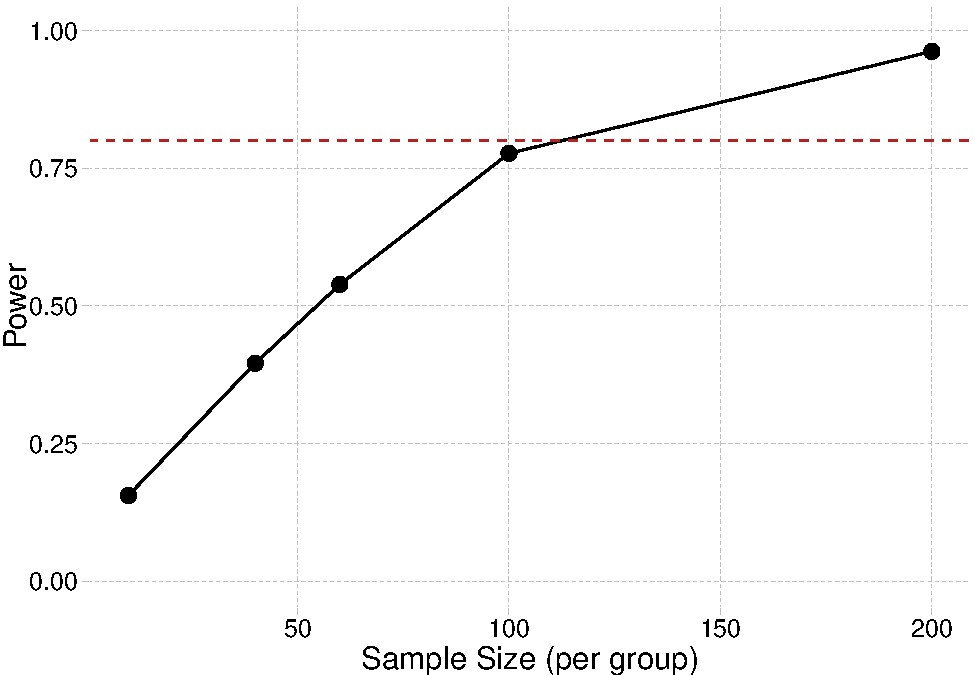
\includegraphics{paper-new_files/figure-latex/unnamed-chunk-28-1} 

}

\caption{ }\label{fig:unnamed-chunk-28}
\end{figure}

\normalsize

\subsection{Disclaimer about the functions}\label{disclaimer-about-the-functions}

The current paper proposed a simplified way with some functions to generate ordinal data. For more complex simulations such as simulating correlated ordinal data the \texttt{simstudy} package \url{https://kgoldfeld.github.io/simstudy/articles/ordinal.html} proposed a very comprehensive set of data simulation function also for ordinal data.

\newpage

\section{References}\label{references}

\phantomsection\label{refs}
\begin{CSLReferences}{1}{0}
\bibitem[\citeproctext]{ref-Agresti2010-rz}
Agresti, A. (2010). \emph{Analysis of ordinal categorical data}. Hoboken, NJ, USA: John Wiley \& Sons, Inc. \url{https://doi.org/10.1002/9780470594001}

\bibitem[\citeproctext]{ref-Burkner2019-aw}
Bürkner, P.-C., \& Vuorre, M. (2019). Ordinal regression models in psychology: A tutorial. \emph{Advances in Methods and Practices in Psychological Science}, \emph{2}, 77--101. \url{https://doi.org/10.1177/2515245918823199}

\bibitem[\citeproctext]{ref-Carifio2008-qd}
Carifio, J., \& Perla, R. (2008). Resolving the 50-year debate around using and misusing likert scales. \emph{Medical Education}, \emph{42}, 1150--1152. \url{https://doi.org/10.1111/j.1365-2923.2008.03172.x}

\bibitem[\citeproctext]{ref-Carifio2007-kk}
Carifio, J., \& Perla, R. J. (2007). Ten common misunderstandings, misconceptions, persistent myths and urban legends about likert scales and likert response formats and their antidotes. \emph{Journal of Social Sciences}, \emph{3}, 106--116. \url{https://doi.org/10.3844/jssp.2007.106.116}

\bibitem[\citeproctext]{ref-Christensen2019-cz}
Christensen, R. H. B. (2019). \emph{Ordinal---regression models for ordinal data}.

\bibitem[\citeproctext]{ref-Cliff1996-qo}
Cliff, N. (1996). Answering ordinal questions with ordinal data using ordinal statistics. \emph{Multivariate Behavioral Research}, \emph{31}, 331--350. \url{https://doi.org/10.1207/s15327906mbr3103_4}

\bibitem[\citeproctext]{ref-Cliff2016-ck}
Cliff, Norman. (2016). \emph{Ordinal methods for behavioral data analysis}. London, England: Psychology Press.

\bibitem[\citeproctext]{ref-Cox1995-ur}
Cox, C. (1995). Location-scale cumulative odds models for ordinal data: A generalized non-linear model approach. \emph{Statistics in Medicine}, \emph{14}, 1191--1203. \url{https://doi.org/10.1002/sim.4780141105}

\bibitem[\citeproctext]{ref-DeCarlo1998-ay}
DeCarlo, L. T. (1998). Signal detection theory and generalized linear models. \emph{Psychological Methods}, \emph{3}, 186--205. \url{https://doi.org/10.1037/1082-989X.3.2.186}

\bibitem[\citeproctext]{ref-DeCarlo2010-lj}
DeCarlo, L. T. (2010). On the statistical and theoretical basis of signal detection theory and extensions: Unequal variance, random coefficient, and mixture models. \emph{Journal of Mathematical Psychology}, \emph{54}, 304--313. \url{https://doi.org/10.1016/j.jmp.2010.01.001}

\bibitem[\citeproctext]{ref-Delacre2017-qy}
Delacre, M., Lakens, D., \& Leys, C. (2017). Why psychologists should by default use welch's \emph{t}-test instead of student's \emph{t}-test. \emph{International Review of Social Psychology}, \emph{30}, 92. \url{https://doi.org/10.5334/irsp.82}

\bibitem[\citeproctext]{ref-Faraggi2003-hm}
Faraggi, D., Izikson, P., \& Reiser, B. (2003). Confidence intervals for the 50 per cent response dose. \emph{Statistics in Medicine}, \emph{22}, 1977--1988. \url{https://doi.org/10.1002/sim.1368}

\bibitem[\citeproctext]{ref-Gelman2020-tg}
Gelman, A., Hill, J., \& Vehtari, A. (2020). \emph{Regression and other stories}. Cambridge University Press. \url{https://doi.org/10.1017/9781139161879}

\bibitem[\citeproctext]{ref-Green1966-gy}
Green, D. M., Swets, J. A., \& Others. (1966). \emph{Signal detection theory and psychophysics} (Vol. 1, pp. xi, 455--xi, 455). Oxford, England: Wiley New York.

\bibitem[\citeproctext]{ref-Jamieson2004-xf}
Jamieson, S. (2004). Likert scales: How to (ab)use them. \emph{Medical Education}, \emph{38}, 1217--1218. \url{https://doi.org/10.1111/j.1365-2929.2004.02012.x}

\bibitem[\citeproctext]{ref-Kemp2021-dj}
Kemp, S., \& Grace, R. C. (2021). Using ordinal scales in psychology. \emph{Methods in Psychology (Online)}, \emph{5}, 100054. \url{https://doi.org/10.1016/j.metip.2021.100054}

\bibitem[\citeproctext]{ref-Knoblauch2012-to}
Knoblauch, K., \& Maloney, L. T. (2012). \emph{Modeling psychophysical data in r}. New York, NY: Springer New York. \url{https://doi.org/10.1007/978-1-4614-4475-6}

\bibitem[\citeproctext]{ref-Kruschke2015-re}
Kruschke, J. K. (2015). \emph{Doing bayesian data analysis}. \url{https://doi.org/10.1016/c2012-0-00477-2}

\bibitem[\citeproctext]{ref-Liddell2018-wu}
Liddell, T. M., \& Kruschke, J. K. (2018). Analyzing ordinal data with metric models: What could possibly go wrong? \emph{Journal of Experimental Social Psychology}, \emph{79}, 328--348. \url{https://doi.org/10.1016/j.jesp.2018.08.009}

\bibitem[\citeproctext]{ref-Likert1932-xw}
Likert, R. (1932). A technique for the measurement of attitudes. \emph{Archives of Psychology}, \emph{22}, 55. Retrieved from \url{https://psycnet.apa.org/record/1933-01885-001}

\bibitem[\citeproctext]{ref-Liu2023-bp}
Liu, A., He, H., Tu, X. M., \& Tang, W. (2023). On testing proportional odds assumptions for proportional odds models. \emph{General Psychiatry}, \emph{36}, e101048. \url{https://doi.org/10.1136/gpsych-2023-101048}

\bibitem[\citeproctext]{ref-McCullagh1980-cw}
McCullagh, P. (1980). Regression models for ordinal data. \emph{Journal of the Royal Statistical Society}, \emph{42}, 109--127. \url{https://doi.org/10.1111/j.2517-6161.1980.tb01109.x}

\bibitem[\citeproctext]{ref-Rigby2005-ko}
Rigby, R. A., \& Stasinopoulos, D. M. (2005). Generalized additive models for location, scale and shape. \emph{Journal of the Royal Statistical Society. Series C, Applied Statistics}, \emph{54}, 507--554. \url{https://doi.org/10.1111/j.1467-9876.2005.00510.x}

\bibitem[\citeproctext]{ref-Robitzsch2020-la}
Robitzsch, A. (2020). Why ordinal variables can (almost) always be treated as continuous variables: Clarifying assumptions of robust continuous and ordinal factor analysis estimation methods. \emph{Frontiers in Education}, \emph{5}, 589965. \url{https://doi.org/10.3389/feduc.2020.589965}

\bibitem[\citeproctext]{ref-Sanchez-Meca2003-ji}
Sánchez-Meca, J., Marín-Martínez, F., \& Chacón-Moscoso, S. (2003). Effect-size indices for dichotomized outcomes in meta-analysis. \emph{Psychological Methods}, \emph{8}, 448--467. \url{https://doi.org/10.1037/1082-989X.8.4.448}

\bibitem[\citeproctext]{ref-Schad2020-ht}
Schad, D. J., Vasishth, S., Hohenstein, S., \& Kliegl, R. (2020). How to capitalize on a priori contrasts in linear (mixed) models: A tutorial. \emph{Journal of Memory and Language}, \emph{110}, 104038. \url{https://doi.org/10.1016/j.jml.2019.104038}

\bibitem[\citeproctext]{ref-Stanislaw1999-jr}
Stanislaw, H., \& Todorov, N. (1999). Calculation of signal detection theory measures. \emph{Behavior Research Methods, Instruments, \& Computers: A Journal of the Psychonomic Society, Inc}, \emph{31}, 137--149. \url{https://doi.org/10.3758/bf03207704}

\bibitem[\citeproctext]{ref-Stevens1946-te}
Stevens, S. S. (1946). On the theory of scales of measurement. \emph{Science (New York, N.Y.)}, \emph{103}, 677--680. \url{https://doi.org/10.1126/science.103.2684.677}

\bibitem[\citeproctext]{ref-Tutz1990-fe}
Tutz, Gerhard. (1990). Sequential item response models with an ordered response. \emph{The British Journal of Mathematical and Statistical Psychology}, \emph{43}, 39--55. \url{https://doi.org/10.1111/j.2044-8317.1990.tb00925.x}

\bibitem[\citeproctext]{ref-Tutz2022-dg}
Tutz, Gerhard. (2022). Ordinal regression: A review and a taxonomy of models. \emph{Wiley Interdisciplinary Reviews. Computational Statistics}, \emph{14}. \url{https://doi.org/10.1002/wics.1545}

\bibitem[\citeproctext]{ref-Tutz2017-de}
Tutz, G., \& Berger, M. (2017). Separating location and dispersion in ordinal regression models. \emph{Econometrics and Statistics}, \emph{2}, 131--148. \url{https://doi.org/10.1016/j.ecosta.2016.10.002}

\bibitem[\citeproctext]{ref-Tutz2020-xq}
Tutz, Gerhard, \& Berger, M. (2020). Non proportional odds models are widely dispensable -- sparser modeling based on parametric and additive location-shift approaches. \emph{arXiv {[}Stat.ME{]}}. Retrieved from \url{http://arxiv.org/abs/2006.03914}

\end{CSLReferences}


















\end{document}
